%!TEX root = ../aluno.tex

\ifnum\aluno=1
\renewcommand\chapterillustration{./abertura-cartografia}
\else
\renewcommand\chapterillustration{./abertura-cartografia-professor}
\fi

\renewcommand\chapterwhat{Projeções cartográficas. Classificação das projeções cartográficas quanto à superfície de projeção (planas, cônicas e cilíndricas) e quanto as propriedades (equivalentes, equidistantes, conformes e afiláticas).}
\renewcommand\chapterbecause{Projeções cartográficas são projeções da superfície terrestre no plano que possibilitam a visualização de uma área muito grande em um único local ( folha de papel, tela de computador ou dispositivo móvel). Essas projeções tornam possível, por exemplo, o planejamento de rotas ou organizações territoriais de um país inteiro em cima de uma mesa. Existem diferentes tipos de projeções e cada uma possui algum tipo de distorção (em relação a área, ângulo ou distância). As projeções cartográficas mais conhecidas são as cônicas, planas e cilíndricas, portanto serão a essas que daremos ênfase no capítulo.}
\chapter{Projeções Cartográficas}



\mbox{}\thispagestyle{empty}\clearpage

\thispagestyle{empty}

\begin{center}
Projeto: LIVRO ABERTO DE MATEMÁTICA

\noindent \begin{tabular}{lcccr}

\includegraphics[scale=.15]{impa}& \quad\quad& 
\includegraphics[width=3cm]{logo} & \quad\quad& 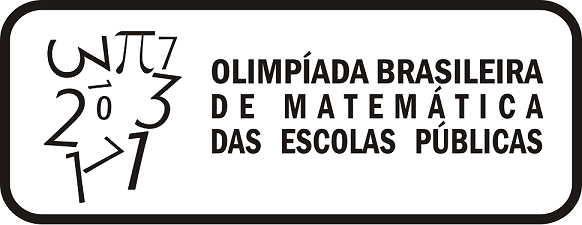
\includegraphics[scale=.24]{obmep} 
\end{tabular}
\end{center}

\vspace*{.3cm}

Cadastre-se como colaborador no site do projeto: \url{umlivroaberto.com}

Versão digital do capítulo:

\url{https://www.umlivroaberto.org/BookCloud/Volume_1/master/view/AF107.html}


\begin{tabular}{p{.15\textwidth}p{.7\textwidth}}
Título: & Projeções Cartográficas\\
\\
Ano/ Versão: & 2020 / versão 0.2 de \today\\
\\
Editora & Instituto Nacional de Matem\'atica Pura e Aplicada (IMPA-OS)\\
\\
Realização:& Olimp\'iada Brasileira de Matem\'atica das Escolas P\'ublicas (OBMEP)\\
\\
Produção:& Livro Aberto\\
\\
Coordenação:& Fabio Simas e Augusto Teixeira (livroaberto@impa.br)\\
\\
  Autores: & Carmen Vieira Mathias (UFSM)\\
             & Lucas Schimith Zanon (SEDUC - RS)\\
\\
Revisão: &  Lhaylla Crissaff (UFF) \\
\\
Design: & Andreza Moreira (Tangentes Design) \\
\\
  Ilustrações: & --- \\ 
\\
Gráficos: & Beatriz Cabral e Tarso Caldas (Licenciandos da UNIRIO)\\
\\
  Capa: & Foto de Clay Banks, no Unsplash \\
  & \url{https://unsplash.com/photos/b5S4FrJb7yQ} \\
\end{tabular}
\vspace{.5cm}


\begin{figure}[b]
\begin{minipage}[l]{5cm}
\centering

{\large Licença:}

  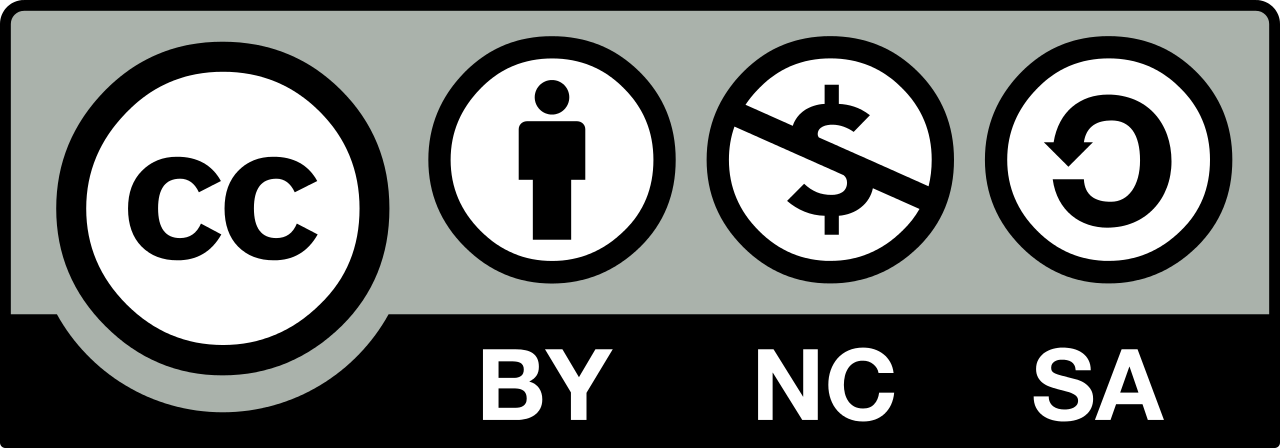
\includegraphics[width=3.5cm]{cc-by-nc-sa}
\end{minipage}\hfill
\begin{minipage}[c]{5cm}
\centering
{\large Desenvolvido por}

%
\includegraphics[width=2.5cm]{logo-associacao.jpg}
\end{minipage}
\begin{minipage}[r]{5cm}
\centering

{\large Patrocínio:}
  \vspace{1em}
  
\includegraphics[width=3.5cm]{itau}
\end{minipage}
\end{figure}

\mainmatter

\begin{apresentacao}{Habilidades e pré-requisitos}
{

Neste capítulo contempla-se a seguinte habilidade da versão homologada da Base Nacional Comum Curricular (BNCC) \citep{BNCC2018} para o ensino médio:

\begin{habilities}{EM13MAT509}
Investigar a deformação de ângulos e áreas provocada pelas diferentes projeções usadas em Cartografia (como a cilíndrica e a cônica), com ou sem suporte de tecnologia digital.
\end{habilities}

 
As habilidades (conforme a versão homologada da BNCC para o ensino fundamental) consideradas como pré-requisitos para o entendimento desse capítulo são:

\begin{habilities}{EF03MA16}
Reconhecer figuras congruentes, usando sobreposição e desenhos em malhas quadriculadas ou triangulares, incluindo o uso de tecnologias digitais.
\tcbsubtitle{EF05MA14} Utilizar e compreender diferentes representações para a localização de objetos no plano, como mapas, células em planilhas eletrônicas e coordenadas geográficas, a fim de desenvolver as primeiras noções de coordenadas cartesianas.
\tcbsubtitle{EF09MA13} Demonstrar relações métricas do triângulo retângulo, entre elas o teorema de Pitágoras, utilizando, inclusive, a semelhança de triângulos.
\tcbsubtitle{EF03GE06}Identificar e interpretar imagens bidimensionais e tridimensionais em diferentes tipos de representação cartográfica.
\tcbsubtitle{EF09GE15}Comparar e classificar diferentes regiões do mundo com base em informações populacionais, econômicas e socioambientais representadas em mapas temáticos e com diferentes projeções cartográficas.
\end{habilities}


Considera-se também como pré-requisitos para o entendimento desse capítulo unidade, as seguintes habilidades do ensino médio, conforme \cite{BNCC2018}:
\begin{habilities}{EM13MAT403}
Analisar e estabelecer relações, com ou sem apoio de tecnologias digitais, entre as representações de funções exponencial e logarítmica expressas em tabelas e em plano cartesiano, para identificar as características fundamentais (domínio, imagem, crescimento) de cada função.
\tcbsubtitle{EM13MAT308} Aplicar as relações métricas, incluindo as leis do seno e do cosseno ou as noções de congruência e semelhança, para resolver e elaborar problemas que envolvem triângulos, em variados contextos.
\end{habilities}

\subsection{Tópicos abordados na unidade}
Nessa unidade serão abordados os seguintes assuntos:
\begin{itemize}
\item Coordenadas geográficas: conceito, elementos e exemplos de utilização.
\item Projeções cartográficas: classificação da projeção cartográfica dependendo da superfície de projeção, da deformação e do ponto de vista.
\end{itemize}
	

Considerando a habilidade EM13MAT509 citada anteriormente, nesse capítulo tem-se os seguintes
\begin{habilities}{Objetivos}
\begin{itemize}
\item reconhecer as projeções cartográficas de acordo com a superfície de projeção;
\item compreender que ocorrem distorções de área, formas ou distâncias ao realizar uma projeção cartográfica. 
\end{itemize}
\end{habilities}

\subsection{Abordagem adotada no capítulo}

Conforme listado nos pré-requisitos, observa-se que a BNCC  apresenta as projeções cartográficas como parte de uma das habilidades para a disciplina de Geografia.

\textit{"(EF09GE15) Comparar e classificar diferentes regiões do mundo com base em informações populacionais, econômicas e socioambientais representadas em mapas temáticos e com diferentes projeções cartográficas."{} \citep[p. 395]{BNCC2018}}

O mesmo documento aborda o tema Cartografia, para o ensino fundamental, na unidade temática formas de representação e pensamento espacial, na disciplina de Geografia. Nesse contexto, 
\textit{[...] espera-se que, no decorrer do ensino fundamental, os alunos tenham domínio da leitura e elaboração de mapas e gráficos, iniciando-se na alfabetização cartográfica. Fotografias, mapas, esquemas, desenhos, imagens de satélites, audiovisuais, gráficos, entre outras alternativas, são frequentemente utilizados no componente curricular (p.363). }

Observa-se que a BNCC para o ensino fundamental não trata do tema projeções cartográficas na disciplina de Matemática, porém o faz para o ensino médio, como uma habilidade a ser atingida (EM13MAT509 citada anteriormente).  Ao examinar os Parâmetros Curriculares Nacionais (PCN) \citep{PCN} não foram encontradas menções ao termo projeções cartográficas, apenas aos termos "cartografia"{}e "cartográfica"{}nos documentos de orientação para a disciplina de Geografia. 

Há inúmeros trabalhos dedicados aos desafios do ensino de projeções cartográficas. Ao considerar os métodos que usamos para educar os alunos sobre as projeções cartográficas \cite{Downs}  examinaram os desafios cognitivos por trás do conceito de projeções e superfícies desenvolvíveis( são aquelas obtidas pela deformação de um plano sem que esse seja esticado, por exemplo o cone, o cilindro o próprio plano). Eles descobriram que muitos indivíduos em idade universitária não têm habilidades cognitivas e espaciais suficientes para compreender as projeções geométricas em perspectiva. Portanto, esses alunos não seriam capazes de compreender efetivamente as projeções cartográficas ensinadas usando projeções geométricas em perspectiva. Nesse sentido é muito importante que o aluno tenha conhecimento sobre projeções e perspectivas, que é tema do capítulo de mesmo nome do Livro Aberto de Matemática.

 Sobre as dificuldades em compreender projeções cartográficas, \cite{Olson} sugere que os alunos  precisam  tornar-se “detetives visuais” e aprender a ler mais de perto as pistas na gratícula (rede de linhas de latitude e longitude sobre as quais o mapa é desenhado) do mapa.

Enquanto \cite{Downs} e \cite{Olson} focaram em como os alunos aprendem sobre projeções cartográficas, \cite{Battersby} examinaram como os alunos aplicam o conhecimento de projeções cartográficas na avaliação de distorções. Uma descoberta deste estudo é uma dependência substancial nas distorções que aparecem na Projeção Cartográfica Mercator (por exemplo, as distorções que ocorrem na Groenlândia, Antártica e nas regiões polares) para explicar a distorção que ocorre nas outras projeções cartográficas incluídas no estudo. \cite{Battersby} afirma que mesmo quando uma projeção cartográfica é familiar, a maioria das pessoas tem dificuldade em perceber as distorções existentes.

Ao pesquisar sobre dificuldades para ensinar projeções cartográficas em artigos de língua portuguesa, existem muitos relatos sobre os obstáculos que os estudantes apresentam no processo de aprendizagem dos conceitos relativos a alfabetização cartográfica, como por exemplo \cite{Almeida}, \cite{Lunkes} e \cite{Ludwig}. Nesses relatos as projeções cartográficas são mencionadas como algo abstrato e difícil de ser ensinado. Segundo \cite{Lunkes} os alunos trazem muitas deficiências sobre o tema Cartografia e possuem dificuldades na leitura e na interpretação de um mapa, portanto possuem dificuldades para uma leitura de mundo. Conforme \cite{Ludwig} a Cartografia ensinada na escola,  muitas vezes, é entendida como sendo apenas uma técnica ou um conjunto de conteúdos, como escala, fusos horários, coordenadas geográficas, projeções cartográficas, entre outros, que são trabalhados sem muita relação dentro com outros tópicos da disciplina de Geografia e de outras disciplinas. \cite{Lunkes} apresenta uma lista de dificuldades encontradas pelos professores de Geografia, no ensino de Cartografia. Como projeções cartográficas é um dos conteúdos incluso nesse tema, acreditamos que você professor, ao trabalhar esse capítulo, possa perceber as mesmas dificuldades, a saber:

\begin{itemize}
\item a dificuldade dos alunos que chegam ao ensino médio para dominarem alguns conceitos básicos ;
\item  diferença de conhecimentos básicos sobre escala, coordenadas, legenda, etc. entre alunos da mesma série, uma vez que eles chegam ao ensino médio, vindo de diversas escolas;
\item  falta de material e ou um espaço que possua um acervo de mapas, maquetes e globos;

\item a carga horária disponível e pouca possibilidade de construção de um material concreto com os alunos; 

\item a própria deficiência na formação do professor quanto ao conteúdo projeções cartográficas no ensino de Matemática.
\end{itemize}



Procurando realizar uma conexão entre diferentes contextos e disciplinas, a abordagem desse capítulo está fundamentada na metodologia de investigação matemática. Justifica-se essa escolha, pois conforme \citet[p. 2]{Ponte} \textit{"em contextos de ensino, aprendizagem ou formação, investigar não significa necessariamente lidar com problemas na fronteira do conhecimento nem com problemas de grande dificuldade. Significa, apenas, trabalhar a partir de questões que nos interessam e que se apresentam inicialmente confusas, mas que conseguimos clarificar e estudar de modo organizado."{}}

\citet[p. 23]{Ponte1} \textit{sustentam o uso dessa metodologia como atividades de ensino-aprendizagem, que permitam o espírito da atividade matemática genuína}. Nesse sentido, conforme os autores, o aluno será capaz de formular conjecturas, prová-las ou refutá-las, além de apresentar os resultados obtidos durante o processo e a discuti-los junto aos demais colegas e ao professor.

Ainda sobre realizar investigações, \citet[p. 5]{Braumann} afirma que 

\textit{Aprender matemática não é simplesmente compreender a matemática já feita, mas ser capaz de fazer investigação de natureza matemática (ao nível adequado a cada grau de ensino). Só assim se pode perceber o que é a matemática e a sua utilidade na compreensão do mundo e na intervenção sobre o mundo. Só assim se pode realmente dominar os conhecimentos adquiridos. Só assim se pode ser inundado pela paixão ‘detetivesca’ indispensável à verdadeira fruição da matemática. Aprender matemática sem forte intervenção da sua faceta investigativa é como tentar aprender a andar de bicicleta vendo os outros andar e recebendo informação sobre como o conseguem. Isso não chega. Para verdadeiramente aprender é preciso montar a bicicleta e andar, fazendo erros e aprendendo com eles.} 

Ou seja, o fazer matemática está intrinsecamente conectado com a sua investigação. Acredita-se que não é possível fazer matemática sem praticá-la, mas essa prática não é necessariamente a prática mecanizada, comumente realizada no cotidiano escolar. Nesse sentido é que esse capítulo foi pensado pois os alunos ao realizarem uma atividade de investigação matemática, a compreensão dos conteúdos poderá ocorrer de uma forma natural. 

\subsection{Orientações sobre o uso do material}

Esse material é dividido em seções do tipo Explorando, Organizando, Praticando, Exercícios e Para Saber Mais. As seções Explorando, Organizando e Praticando foram pensadas para o desenvolvimento em sala. As seções denominadas Para Saber Mais são de caráter opcional, ao omiti-las não irá prejudicar o desenvolvimento das demais atividades. Apenas observamos que em geral elas exploram aspectos interessantes do conteúdo. A seção denominada Exercícios contém atividades que devem ser desenvolvidas pelos estudantes fora do horário de aula. 

O material foi planejado para ser desenvolvido em 3 semanas ou 4 semanas com três horas aula por semana e, para isso, seria necessário o desenvolvimento das atividades de modo eficiente pelos estudantes. Você  professor pode suprimir  algumas das atividades (ou até mesmo as duas primeiras seções) se julgar que a turma já possui nível de maturidade adequado nos respectivos assuntos.

O capítulo se inicia com atividades que procuram levar o aluno a perceber que as projeções cartográficas são formas de representar a superfície terrestre e que esse assunto tem relação direta com a disciplina de Matemática. Para isto, a primeira atividade inspirada na investigação realizada em \citep{Nussbaum} tem por objetivo que o aluno reconheça sua posição na superfície terrestre. Isso é importante, pois conforme os autores da pesquisa, não possuir tal percepção pode ser um obstáculo epistemológico na compreensão de outros conteúdos, como por exemplo, a projeção dessa superfície em um plano. 

Acredita-se que a atividade pode oportunizar uma discussão sobre a relação existente entre diferentes disciplinas, visto que, conforme comentado anteriormente o tema projeção cartográfica deve ter sido abordado no ensino fundamental na disciplina de Geografia. Nesse mesmo sentido, são propostas outras atividades que tem por objetivo fazer com que o aluno  reconheça que existem diferentes formas de representar o mesmo objeto e com isso perceba a necessidade das projeções cartográficas. 

A segunda seção, aborda aspectos relativos as coordenadas geográficas e explora a necessidade de conhecê-las para compreender as distorções que ocorrem, por exemplo, nos paralelos e meridianos ao realizar uma  projeção cartográfica.

A terceira seção trata da impossibilidade de planificar a superfície terrestre. O objetivo dessas atividades é fazer com que o aluno entenda que ocorrem deformações no processo de “transformar” uma superfície esférica em um plano. Nessa seção, que é composta por dois blocos do tipo Explorando e Organizando o aluno tem contato com algumas projeções cartográficas mais comuns, onde são explorados alguns aspectos em termos de deformações ocorridas no processo. Essa seção apresenta os conceitos mais  importantes do capítulo (projeção cartográfica e a classificação destas quanto as distorções) e apresenta no Para Saber Mais um exemplo que poderá auxiliar os estudantes a compreender o conceito de projeção cartográfica em termos matemáticos. 

Observamos que a discussão quanto as deformação provocadas pelas diferentes projeções usadas em Cartografia não se esgotam nessa seção, elas serão retomadas a partir de exemplos na próxima seção do capítulo.

Os principais tipos de projeções cartográficas, são explorados na quinta seção, que é composta por três blocos do tipo Explorando e Organizando. É nessa seção que o aluno irá compreender, a partir de atividades práticas, quais os tipos de projeções são as mais comuns e por que as deformações ocorrem.

Optamos por escrever um capítulo de reconhecimento, não de cálculos. Pois, para compreender os processos matemáticos envolvidos na maioria das projeções cartográficas são necessários conceitos de cálculo diferencial e integral, que não fazem parte do escopo do nível de ensino que os alunos se encontram.

}
\end{apresentacao}

\def\currentcolor{session1}
\begin{texto}
{
	\subsection{Explorando: O Problema do Cartógrafo}

	\paragraph{Objetivo geral}
	\begin{itemize}
	\item Reconhecer que a superfície terrestre pode ser representada por uma esfera.
	\end{itemize}

	Para cumprir tal objetivo são propostas 3 atividades:
	\begin{itemize}
	\item A primeira atividade inspirada nas investigações realizadas em \citep{Nussbaum} e \citep{Nardi}  tem por \textbf{objetivo} que o \textbf{aluno reconheça sua posição na superfície terrestre}. Isso é importante, pois conforme os autores da pesquisa, não possuir tal percepção pode ser um obstáculo epistemológico na compreensão de outros conteúdos, como por exemplo, a projeção dessa superfície em um plano. Acredita-se que a atividade pode oportunizar uma discussão sobre a relação existente entre diferentes disciplinas, visto que, conforme comentado anteriormente, o tema projeção cartográfica deve ter sido abordado no ensino fundamental na disciplina de Geografia.
	\item A segunda atividade tem por \textbf{objetivo} fazer com que o aluno \textbf{reconheça que a superfície do planeta Terra pode ser aproximada por uma esfera}. A ideia aqui é proporcionar ao aluno uma experiência que o faça pensar na diferença de uma representação plana e uma representação espacial. Além disso, acredita-se ser uma oportunidade para que, você professor, possa verificar as principais ideias dos alunos sobre a forma da Terra. A pesquisa realizada em \citep{Nussbaum1} deixa claro que a ideia de a Terra ser uma superfície do tipo esférico não é óbvia por si mesma. Segundo os autores, é um conceito construído e que interfere na constituição de outras noções. Observa-se que essa pode ser uma oportunidade para discutir o capítulo como um todo, questionando os alunos sobre a ideia de a Terra ser "plana". Faça-os perceber que, se a Terra fosse plana, não seria necessário pensar em projeções cartográficas, bastaria representá-la em uma escala reduzida.
	\item Já a terceira atividade tem \textbf{por objetivo} fazer com que o aluno \textbf{reconheça que existem diferentes formas de comunicar a mesma ideia}. Nessa atividade é muito importante que os alunos reconheçam o terceiro homem como alguém que está fazendo um mapa (geógrafo, cartógrafo ou topógrafo).
	\end{itemize}
}
\end{texto}
\explore{O problema do cartógrafo}\label{cart_1}

Alguns autores afirmam que a Cartografia (do grego \textit{chartis} = mapa e \textit{graphein} = escrita) é, ao mesmo tempo, ciência e arte.  A arte é evidente, pois está associada à estética, clareza, harmonia e simplicidade. Especialmente em velhos mapas históricos (\hyperref[mapa_ant]{Figura \ref{mapa_ant}}), nos quais quem o fazia, preenchia os oceanos com figuras de velhos barcos a vela, e outros tipos de desenhos.

\begin{figure}[H]
\centering
\includegraphics[height=66mm]{{mapa_ant}.png}
\caption{Mapa antigo. \\ Figura de \href{https://stock.adobe.com/br/images/old-vintage-world-map/178102789}{pingebat, no Adobe Stock}}
\label{mapa_ant}
\end{figure}


Já a Cartografia como ciência vem do conhecimento de como comunicar, ou seja, quais instrumentos e técnicas devem ser utilizados para que a realidade seja representada com maior exatidão, utilizando conceitos da Astronomia e da Matemática. 
Assim, o cartógrafo (profissional dedicado à Cartografia e à produção de mapas) precisa conhecer aspectos artísticos e técnicos para realizar seu trabalho.

Nas atividades a seguir, vamos pensar um pouco sobre o que esse profissional precisa conhecer para fazer uma representação plana da superfície do planeta Terra.

\clearpage

{\vspace{2em}
\begin{objectives}{O astronauta}
{
\begin{itemize}
\item Reconhecer sua posição na superfície terrestre.

\end{itemize}
}
{1}{0}
\end{objectives}
\begin{sugestions}{O astronauta}
{
	\begin{itemize}
	\item \textbf{Conceitos abordados}: Posição de um corpo e o  lugar do corpo no espaço.
	
	\item \textbf{Organização em sala de aula}: Nesta atividade, que sugere-se ser feita de forma individual, o aluno deve ilustrar o que é solicitado. Após primeiro momento, sugere-se que os alunos organizem-se em duplas ou trios e comparem as ilustrações. A discussão em grupos contribuirá para a percepção de cada aluno sobre o seu lugar no espaço e os pontos de referência utilizados (astronautas, nuvens, lua, etc.).
	\item \textbf{Dificuldades previstas}: Acredita-se que os alunos não terão dificuldades em realizar o desenho, visto que é algo simples e pode ser feito como um esquema. O que pode ocorrer é o aluno desenhar o planeta Terra como algo plano ou não desenhar a Terra.
	\item \textbf{Sugestões gerais}: Para o desenvolvimento da tarefa recomenda-se que sejam entregues folhas de papel aos alunos, pois é interessante que os mesmos guardem seus desenhos para posterior discussão (ver o  \hyperref[organizando-carto]{Organizando - O problema do cartógrafo \ref{organizando-carto}}).
	\item \textbf{Material necessário}: Folhas de papel sulfite.
	\item \textbf{Enriquecimento da discussão}: Acredita-se que a atividade pode oportunizar uma discussão sobre a relação existente entre diferentes disciplinas, visto que, conforme comentado anteriormente, o tema projeção cartográfica deve ter sido abordado no ensino fundamental na disciplina de geografia. Além disso, o professor pode questionar "como é o formato do nosso planeta?"{}ou "o que faz você pensar que a Terra é assim?". Caso o aluno tenha feito um desenho diferente do esperado (conforme consta na resposta) solicite que ele desenhe pessoas em diferentes locais da sua representação da Terra. Caso tenha desenhado a Terra como algo plano, questione "o que aconteceria se saísse de casa e andasse na mesma direção?"{}Questione o aluno "por onde ele vai passar e onde ele vai chegar".
	\end{itemize}
}{1}{0}
\end{sugestions}}


\begin{answer}{O astronauta}
{Apesar da resposta ser pessoal, \cite{Nardi} apontam que  os alunos poderão esboçar  uma das seguintes possibilidades: 
  
 \begin{figure}[H]
	\centering
		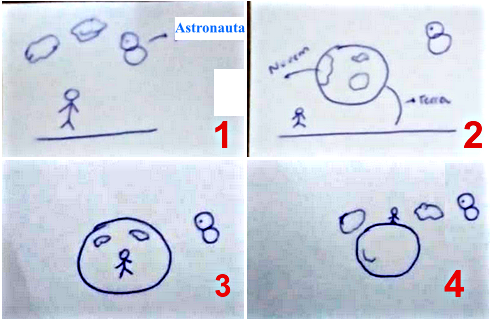
\includegraphics[width=.6\linewidth]{resp_astro}
	\end{figure}
	
Em ilustrações do tipo 1 , a Terra é um plano e os astros estão no "céu"{}que, por sua vez, é paralelo ao "chão". 
No tipo 2, o aluno admite a natureza esférica e espacial da Terra, porém, os objetos soltos próximo à sua superfície caem  para um chão imaginário, no espaço, localizado abaixo do planeta. Nas ilustrações do tipo 3, o aluno concebe o planeta Terra como esférico, porém, o entende como um corpo oco, com os indivíduos vivendo na sua parte interna inferior e as nuvens na parte interna superior. Ilustrações do tipo 4 são as esperadas para o nível de ensino que os alunos estão. }{0}
\end{answer}




\clearmargin
\begin{objectives}{Qual o verdadeiro formato da Terra?}
{
	\begin{itemize}
	\item Reconhecer que o formato do planeta Terra é  tridimensional.
	\item Reconhecer que as figuras (mapas) apresentadas são representações no plano de parte da superfície terrestre.

	\end{itemize}
}{1}{1}
\end{objectives}
\begin{sugestions}{Qual o verdadeiro formato da Terra?}
{
	\begin{itemize}
	\item \textbf{Conceitos abordados}: Rotas, formas planas e formas espaciais.
	\item  \textbf{Organização em sala de aula}: Pode ser feito individual ou em dupla.
	\item \textbf{Material necessário}: Lápis e papel.
	\item \textbf{Enriquecimento da discussão}: Pretende-se que essa atividade  proporcione ao aluno pensar sobre o formato da superfície terrestre. Na \textbf{Parte 1}, sugerimos que o professor enfatize que as distâncias das rotas estão corretas, e permita que a turma debata sobre qual seria o trajeto ideal para a segunda rota, de forma que ela seja tão curta quanto à primeira.	Esta atividade exibe uma pequena falha no aplicativo utilizado. Assim, queremos mostrar ao aluno que os extremos laterais do mapa na realidade estão conectados. Na \textbf{Parte 2}, é importante que seja realizado um debate em torno das respostas dos alunos, pois  ter uma ideia clara do formato do planeta irá auxiliar no entendimento das projeções cartográficas.
	
	\end{itemize}
	
	
	
}{1}{1}
\end{sugestions}
\begin{answer}{Qual o verdadeiro formato da Terra?}
{Parte 1: Visto que na primeira rota é obrigatório passar pela Europa, o trajeto se torna muito maior do que ele se ele apenas atravessasse o pacífico e chegasse ao destino (Nogliki) pelo caminho mais curto. Porém, alguma falha na programação do aplicativo impede de fazer a representação correta, que seria aproximadamente esta:
	\begin{figure}[H]
	\centering
	
	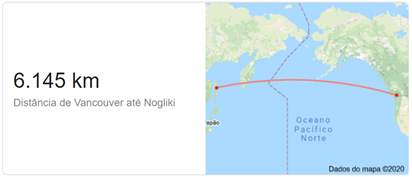
\includegraphics[width=.6\linewidth]{cartografia-professor1}
	\end{figure}

	Parte 2: Resposta pessoal
}{1}
\end{answer}
\begin{objectives}{Observando a paisagem}
{
	\begin{itemize}
	\item Reconhecer que existem diferentes formas de comunicar a mesma ideia.
	\item Entender o conceito de Cartografia.
	\end{itemize}
}{1}{0}
\end{objectives}
\vspace{-.5em}
\begin{sugestions}{Observando a paisagem}
{
	Sugerimos que o professor solicite aos alunos que eles registrem suas respostas e justificativas desta atividade observando a paisagem. Caso as justificativas não apareçam de forma natural, apresente algum dos argumentos do  \hyperref[organizando-carto]{Organizando - O problema do cartógrafo \ref{organizando-carto}}.
	
	\begin{itemize}
	\item \textbf{Organização em sala de aula}: Os alunos podem se organizar em trios, para que a discussão se torne mais rica.
	
	\item \textbf{Dificuldades Previstas}: Nessa atividade é muito importante que os alunos reconheçam o terceiro homem como alguém que está fazendo um mapa (geógrafo, cartógrafo ou topógrafo). Caso isso não ocorra, o porfessor poderá conduzir o estudante a essa resposta, apontando por exemplos, as ferramentas que o terceiro homem está utilizando.
	
	\item \textbf{Enriquecimento da discussão}: Caso o professor já tenha utilizado o capítulo de projeções e perspectivas, sugerimos lembrar os alunos que é possível ter diferentes representações para o mesmo objeto. No referido capítulo, já foi trazido como exemplo a ideia de representar no plano o globo terrestre modelado como uma esfera, onde os autores concluem que tais representações nada mais são do que mapas cartográficos da Geografia, e que a escolha do mapa depende do que se quer comunicar.
	\end{itemize}
}{1}{0}
\end{sugestions}
\begin{answer}{Observando a paisagem}
{
	Apesar da resposta ser pessoal, pois o aluno pode concordar ou não, podemos frisar como o pintor, além de artista, usa técnicas de pintura que são uma forma de ciência. O escritor possui conhecimentos sobre aspectos da linguagem, contudo, a arte está presente na forma da escrita e sua descrição do que enxerga. Por fim, o cartógrafo utiliza diversas ferramentas, mostrando que existe uma precisão necessária (ciência), além de uma arte em suas representações.

}{1}
\end{answer}

\begin{task}{O astronauta}\label{astronauta}

\begin{enumerate}

\item Descreva em palavras a cena ilustrada na \hyperref[carto1]{Figura \ref{carto1}}.

\begin{figure}[H]
\centering
\includegraphics[width=300bp]{{carto1}.jpg}
\caption{O astronauta. \\ Foto de \href{https://unsplash.com/photos/XClNDg9Z9Ag}{Monica Garniga, no Unsplash}}
\label{carto1}
\end{figure}


\item Faça um esboço que ilustre o que você descreveu.
\item Desenhe onde você está nesse esboço.
\item Sinalize onde estão as nuvens no seu esboço.
\item Organizem-se em grupos de três alunos e socializem suas respostas.
\end{enumerate}
\end{task}


\begin{task}{Qual o verdadeiro formato do planeta Terra?}
\label{forma_terra}

\textbf{Parte 1:}  Observe os  mapas ilustrados nas \hyperref[rota1]{Figuras \ref{rota1} e \ref{rota2}}  e responda as questões abaixo:

\begin{figure}[H]
\centering
\includegraphics[width=0.8\textwidth]{{carto_2}.png}
\caption{Rota 1}
\label{rota1}
\end{figure}

\begin{figure}[H]
\centering
\includegraphics[width=0.8\textwidth]{{carto_3}.png}
\caption{Rota 2}
\label{rota2}
\end{figure}

A primeira  rota traçada no aplicativo, possui comprimento aproximado de 18.883 km (dezoito mil, oitocentos e oitenta e três quilômetros), já a segunda rota tem um  comprimento aproximado de 6.192 km (seis mil, cento e noventa e dois quilômetros).

\begin{enumerate}
\item A origem e o destino final das rotas dos dois mapas são iguais ou próximos? Justifique  por que a distância  entre estes dois pontos é tão distinta.
\item Seria possível chegar no destino final por outra rota (justificando a diferença de medidas)? Se sim, qual seria essa rota alternativa?
\item Mesmo sendo origem e destino final da rota diferentes, você acha que a primeira é cerca de três vezes maior? Justifique sua resposta.
\item A representação está equivocada? Se sim, como seria a correta?
\end{enumerate}


\textbf{Parte 2:}
Na sua opinião, qual das imagens ilustradas na \hyperref[planeta]{Figura \ref{planeta}} melhor representa o formato do planeta Terra? Por quê?

\begin{figure}[H]
\centering
\includegraphics[width=0.8\textwidth]{{carto4a}.jpg}
\caption{Representações do planeta Terra}
\label{planeta}
\end{figure}

\end{task}

\begin{task}{Observando a paisagem}
Na \hyperref[paisag]{Figura \ref{paisag}}  três homens estão observando a mesma paisagem. Observe que cada um deles está fazendo suas próprias combinações da arte e da ciência? Você concorda com essa afirmação? Justifique!

\begin{figure}[H]
\centering
\includegraphics[width=0.8\textwidth]{{carto10}.png}
\caption{Observando a paisagem \\ Fonte: \textbf{Anderson (1982)} }
\label{paisag}
\end{figure}


\end{task}



\arrange{O problema do cartógrafo}
\label{organizando-carto} 
Ao observar a \hyperref[paisag]{Figura \ref{paisag}},  é possível pensar que o escritor (pessoa situada no centro da figura) precisa conhecer as normas (a ciência) da construção gramatical e redação. Ou seja, o que ele faz é ciência. Alguns podem dizer que é arte, pois como escritor, é necessário realizar uma seleção das palavras para  expressar verbalmente aquilo que ele percebe visualmente.

O pintor é um artista, por natureza. Porém, provavelmente ele aprendeu nas escolas de arte que estudou os aspectos científicos das tintas, sobre os corantes, a respeito da combinação das cores, como perceber o ambiente, etc. 	
	
A terceira pessoa, pode ser um geógrafo, cartógrafo ou topógrafo. Nesse caso, como cientista, as observações que está realizando são muito importantes. Contudo, está aproveitando seu senso estético para produzir um mapa, que é uma representação plana reduzida de uma dada área do espaço geográfico, que nesse caso, será ao mesmo tempo um resultado artístico e científico.

Observa-se que na Cartografia, a arte inclui o esquema ou o \textit{layout} do desenho, que influi na aparência estética do mapa como um todo. Já a ciência inclui o conhecimento de quais símbolos colocar em um mapa, e quais itens omitir e a noção da projeção a ser utilizada em cada situação. Ou seja, os mapas são uma expressão da necessidade humana de conhecer e representar o seu espaço e como produtos da Cartografia possuem algumas características importantes. Os mapas são imagens gráficas bidimensionais, resultado da aplicação de símbolos gráficos, como cores, ícones, pontos, linhas e outros. 

Alguns desses símbolos gráficos apresentam padronizações, como por exemplo, utilizar a cor azul para representar o mar, utilizar linhas tracejadas para representar ferrovias, aviões para representar aeroportos, etc.  O mar, as ferrovias, os aeroportos são aspectos retratados no mapa em uma determinada escala. 

Por isso, pensamos na atividade “\hyperref[astronauta]{O astronauta}”. Como você descreveu a imagem? Precisou pensar no planeta Terra para descrevê-la? E ao fazer o esboço, o planeta Terra precisou aparecer? Em que momento? Por quê?
Algumas pesquisas mostram que existem diferentes concepções utilizadas para representar o espaço que vivemos e essas noções podem depender da idade da pessoa.

Essa preocupação em descrever a verdadeira forma da Terra, apesar de atualmente ser um assunto recorrente, remonta a Grécia antiga. O principal motivo, naquela época, para esta inquietação estava relacionado com a necessidade de compreender o mundo. 

Por volta do ano 200 antes da era Cristã, um matemático e astrônomo grego chamado Erastóstenes determinou a circunferência terrestre comprovando, de certa forma, que a Terra realmente possuía o formato de uma superfície esférica (\hyperref[esf]{Figura \ref{esf}}), como é explicado no capítulo de Trigonometria. 


\begin{figure}[H]
\centering
\includegraphics[width=0.3\textwidth]{{carto12}.jpg}
\caption{Modelo esférico da Terra. \\ Foto de \href{https://unsplash.com/photos/yEauzeZU6xo}{The New York Public Library, no Unsplash}}
\label{esf}
\end{figure}

No século XVII, o físico inglês Isaac Newton e o matemático holandês Christiaan Huygens alegaram que a superfície terrestre não era esférica pois, possuía um sutil achatamento nos polos. Em função dessa descoberta, passou-se a considerar que a superfície da Terra não é uma esfera perfeita, mas que a figura geométrica mais semelhante a superfície do nosso planeta era o elipsoide de revolução. Um elipsoide de revolução é um sólido geométrico gerado por uma curva (chamada elipse) que gira  em  torno  do  seu  eixo  menor (\hyperref[elipse]{Figura \ref{elipse}}).  

\begin{figure}[H]
\centering
\includegraphics[width=0.4\textwidth]{{carto11}.png}
\caption{Elipsoide de revolução. \\ Fonte: \href{Geogebra}{https://www.geogebra.org/m/dbu5h92x}} 
\label{elipse}
\end{figure}

Porém, pesquisas realizadas no final do século XIX e início do século XX eliminam a hipótese da superfície terreste ser um elipsoide de revolução, pelo contrário, chegou-se à conclusão de que a superfície da Terra possui muitas irregularidades e desta forma, seu formato não tem uma representação matemática muito simples. Buscando contornar esta falta de representação matemática explícita para a superfície da Terra, Johann Carl Friedrich Gauss, matemático alemão, caracterizou-a como um geoide (\hyperref[geoide]{Figura \ref{geoide}}). O geoide é um sólido muito parecido com a esfera, mas possui suaves ondulações e achatado nos polos.

\begin{figure}[H]
\centering
\includegraphics[width=0.35\textwidth]{{carto5}.jpg}
\caption{Geoide. \\ Fonte: \href{https://apod.nasa.gov/apod/ap141215.html}{Astronomy Picture of The Day, Nasa}} 
\label{geoide}
\end{figure}

Para fins didáticos, utiliza-se o o globo terrestre (\hyperref[globo]{Figura \ref{globo}}), que é a representação da superfície da Terra  na forma de uma esfera de tamanho reduzido. No site \href{https://www.leventhalmap.org/digital-exhibitions/bending-lines/interactives/shaded-globe/}{Norman B. Leventhal Map \& Education Center} encontra-se uma versão digital do globo terrestre.


\begin{figure}[H]
\centering
\includegraphics[width=0.4\textwidth]{{carto13}.png}
\caption{Globo terrestre. \\ Foto de \href{https://unsplash.com/photos/9tmrYLRL7Ww}{Subhash Nusetti, no Unsplash}}
\label{globo}
\end{figure}

Em termos cartográficos, em geral, assume-se uma escala média de 1 para 5.000.000, ao representar a Terra como uma esfera. 

Para produzir um mapa, necessitamos de alguns elementos já estudados na disciplina de Geografia, e é sobre isso que trata a próxima seção.

\begin{reflection}
Por que os corpos celestes (sol, lua e planetas, por exemplo) parecem ser todos aproximadamente esféricos? 
\end{reflection}


\begin{reflection}
Na atividade \hyperref[forma_terra]{Qual o verdadeiro formato do planeta Terra?} apresentamos sete imagens, discutimos sobre três. E as outras imagens, também podem ser representações da superfície da Terra?
\end{reflection}



\cleardoublepage

\def\currentcolor{session1}
\begin{objectives}{Que números são esses?}
{
  \begin{itemize}
  \item Reconhecer as coordenadas geográficas e os demais elementos utilizados nas projeções cartográficas.
  
  \end{itemize}
}{1}{1}
\end{objectives}
\begin{sugestions}{Que números são esses?}
{
Acreditamos que os conceitos abordados nessa seção já são de conhecimento dos alunos. Porém, é interessante retomá-los a partir de uma perspectiva diferente, utilizando termos usuais da Matemática. A ideia de localização de um determinado ponto no \textit{Google Maps} é muito intuitiva e simples, porém, caso tenha curiosidade ou alguma dificuldade para realizar a atividade, recomendamos o vídeo \url{https://www.youtube.com/watch?v=zy2cVPdYVRw}, que explica como localizar um ponto no aplicativo. Caso não tenha acesso à internet, é possível adaptar a atividade utilizando um mapa-múndi e um globo terrestre como o da (\hyperref[globo]{Figura \ref{globo}})

\begin{itemize}
\item \textbf{Conceitos abordados}: latitude e longitude.
\item \textbf{Organização em sala de aula}: Essa atividade pode ser realizada em duplas ou pequenos grupos para que ocorram discussões e comparação de respostas. A atividade pode ser realizada em sala de aula, com o uso de dispositivos móveis ou no laboratório de informática. Outra alternativa é que o professor utilizar de um computador e projetar a realização da atividade para a turma.
\item \textbf{Enriquecimento da discussão}: Discuta com os alunos o que eles já sabem sobre mapas. Questione o quão fácil ou difícil seria apontar uma localização em um globo sem usar um sistema de coordenadas. Solicite aos alunos que encontrem pontos de referência com a mesma latitude e longitude de sua localização.
\end{itemize}
}{1}{1}
\end{sugestions}
\begin{answer}{Que números são esses?}
{Exemplo de resposta:

  \textbf{Parte 1}
  \begin{enumerate}
  \item Por exemplo: Ivorá, RS.
  \item ---
  \item --29{,}522321; --53,585332.
  \item Significam a latitude e longitude deste ponto.
  \end{enumerate}
\vspace{\baselineskip}
  \textbf{Parte 2}
  \begin{enumerate}
  \item Fica bem próximo da  cidade do aluno.
  \item Foi parar no meio do oceano Atlântico no final da América do Sul.
  \item Foi para a Ásia Ocidental.
  \item Eles indicam um ponto preciso na superfície da Terra. Na parte 1 seriam as coordenadas da  cidade do aluno.
  \end{enumerate}
}{0}
\end{answer}

\explore{Coordenadas Geográficas}\label{coord_geo}



\begin{task}{Que números são esses?} \label{at_numeros}

\textbf{Parte 1}: Para realizar essa atividade é necessário o uso do aplicativo Google Maps (\url{https://www.google.com/maps}) no dispositivo móvel (tablet ou celular) ou no computador.

\begin{enumerate}
\item Utilize o aplicativo para encontrar sua cidade.
\item Clique ou toque em um ponto qualquer da cidade (insira um “alfinete”). Ao fazer isso, aparecerão alguns números na tela.
\item Copie esses números no seu caderno.
\item Você sabe o que esses números significam?
\end{enumerate}

\textbf{Parte 2}: Para realizar essa atividade é necessário o uso do aplicativo Geogebra (\url{https://www.geogebra.org/m/fzcrw7nm}).
\begin{enumerate}
\item Movimente os controles deslizantes nomeados de latitude e longitude, até obter os números obtidos na Parte 1 (despreze os números após o ponto).
\item Se a ordem dos números for trocada, o que ocorre? Tente descobrir utilizando o aplicativo.
\item Se o sinal for desprezado, o que ocorre? Tente descobrir utilizando o aplicativo.
\item Qual a relação dos valores “latitude” e “longitude” para os números obtidos na Parte 1?
\end{enumerate}

\end{task}


\arrange{Coordenadas Geográficas}
\label{organizando-coord_geo}

Para se determinar uma distância, ou um local qualquer sobre a superfície da Terra, é necessário sempre conhecer alguns elementos básicos. Um sistema de localização, por exemplo, composto pelo nome do Estado, da cidade, do bairro, da rua, número do prédio e do apartamento é suficiente para localizar uma pessoa que habita algum espaço urbano. Mas, se essa pessoa habita um espaço plano sem referências, surgirão obstáculos que impedem a materialização matemática de um sistema assim descrito, ou seja, dificultando sua representação em forma matemática. Para que isso aconteça, é preciso definir um sistema de coordenadas conveniente para registrar uma posição no espaço.  

Na  atividade “\hyperref[at_numeros]{Que números são esses?}” percebemos que existem números associados a diferentes locais da superfície terrestre. Mas de onde eles surgem?
Para representar a posição de um ponto sobre uma superfície (elipsoide, esfera ou plano) usar um sistema de coordenadas é indispensável. Para o plano, um sistema de coordenadas cartesianas $x$ e $y$ é usualmente aplicado, enquanto que para o elipsoide ou a esfera, usualmente empregamos um sistema de coordenadas cartesiano e curvilíneo.

Assim, para que cada ponto da superfície da Terra pudesse ser localizado no mapa, foi criado um sistema de linhas imaginárias chamado Sistema de Coordenadas Geográficas. Existem dois tipos de linhas imaginárias nos mapas e no globo terrestre, os paralelos e os meridianos (\hyperref[parmer]{Figura \ref{parmer}}), que foram criados para facilitar/determinar a localização precisa de qualquer ponto na superfície da Terra. 


\begin{figure}[H]
\centering
\includegraphics[width=0.75\textwidth]{{carto21}.png}
\caption{Paralelos e meridianos.}
\label{parmer}
\end{figure}

Os paralelos são linhas imaginárias que dão uma volta completa em torno da Terra no sentido leste-oeste (\hyperref[paralelos]{Figura \ref{paralelos}}).

\begin{figure}[H]
\centering
\includegraphics[width=0.3\textwidth]{{carto22}.png}
\caption{Paralelos.}
\label{paralelos}
\end{figure}

O principal paralelo, chama-se Linha do Equador. A linha do Equador é o paralelo de referência, correspondendo ao círculo máximo perpendicular ao eixo da Terra e dividindo-a em dois hemisférios, Norte e Sul. Os restantes dos paralelos são círculos menores paralelos ao Equador. Além do Equador, outros paralelos conhecidos são o trópico de câncer, o trópico de capricórnio, o círculo polar ártico e o círculo polar antártico (\hyperref[ppar]{Figura \ref{ppar}}).

\begin{figure}[H]
\centering
\includegraphics[width=0.4\textwidth]{{carto23}.png}
\caption{Principais paralelos.}
\label{ppar}
\end{figure}

\begin{knowledge}
A cidade de Macapá  é a única capital do Brasil cortada pela linha do Equador? Lá existe um estádio de futebol chamado Zerão cuja linha central do meio de campo é a linha imaginária do Equador, assim um time joga no hemisfério Norte e outro no hemisfério Sul. Interessante, né?  
\end{knowledge}
 
Os meridianos são linhas imaginárias que cortam a Terra do polo norte ao polo sul. Eles são círculos máximos que passam pelos polos e são perpendiculares ao Equador. A metade de um meridiano, que vai de polo a polo, chama-se  semi meridiano. O meridiano de referência, que divide a Terra em oeste e leste,  adotado desde 1884 é o semimeridiano de Greenwich (\hyperref[mer]{Figura \ref{mer}}) , que passa pelo observatório astronômico de mesmo nome na Grã Bretanha.

\begin{figure}[H]
\centering
\includegraphics[width=0.35\textwidth]{{carto24}.png}
\caption{Meridianos.}
\label{mer}
\end{figure}


Um determinado ponto da superfície da Terra é obtida pela interseção de um meridiano e um paralelo (\hyperref[ponto]{Figura \ref{ponto}}). 

\begin{figure}[H]
\centering
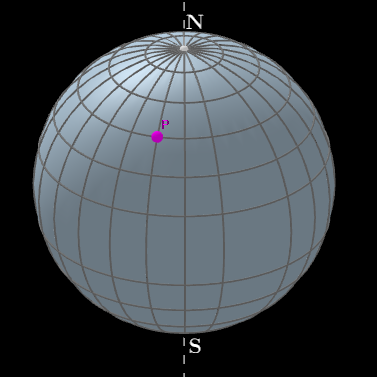
\includegraphics[width=0.4\textwidth]{ponto.png}
\caption{Ponto na superfície da Terra.}
\label{ponto}
\end{figure}


Em um sistema de coordenadas geográficas, cada ponto na superfície da Terra é identificado por dois ângulos (expressos habitualmente em graus, minutos e segundos): longitude ($\varphi$) e a  latitude ($\lambda$) (\hyperref[latlon]{Figura \ref{latlon}}).


\begin{figure}[H]
\centering
\includegraphics[width=0.4\textwidth]{{carto25}.png}
\caption{Latitude e longitude.}
\label{latlon}
\end{figure}



A latitude ($\lambda$) de um lugar é a amplitude do ângulo entre o plano do Equador e o raio que passa por esse lugar (\hyperref[lat]{Figura \ref{lat}}).


\begin{figure}[H]
\centering
\includegraphics[width=0.4\textwidth]{{lat}.png}
\caption{Latitude ($\lambda$).}
\label{lat}
\end{figure}



A  latitude varia de $0^{\circ}$, no Equador a $90^{\circ}$ nos polos Norte (N) ou Sul (S). A latitude quando medida no sentido do polo Norte é chamada Latitude Norte ou Positiva, quando medida no sentido Sul é chamada Latitude Sul ou Negativa. 



A longitude de um lugar é a amplitude do ângulo entre o plano do meridiano desse lugar e o semimeridiano de Greenwich (\hyperref[lon]{Figura \ref{lon}}).


\begin{figure}[H]
\centering
\includegraphics[width=0.4\textwidth]{{lon}.png}
\caption{Longitude ($\varphi$).}
\label{lon}
\end{figure}. 


A longitude varia entre $0^{\circ}$ e $180^{\circ}$ Este (E) ou Oeste (W). A longitude pode ser medida no sentido oeste, quando é chamada Longitude Oeste de Greenwich  ou Negativa. Se medida no sentido este, é denominada Longitude Este de Greenwich ou Positiva.

Os valores de latitude e longitude de um local determinam as coordenadas geográficas do mesmo. O vídeo \url{https://youtu.be/ibE2S8OkNJ8} apresenta mais detalhes sobre essas coordenadas.

 

Por exemplo, a cidade do Rio de Janeiro está localizada a uma latitude de aproximadamente $22^{\circ}$ S  e uma longitude aproximada de $43^{\circ}$ W (\hyperref[rio]{Figura \ref{rio}}).

\begin{figure}[H]
\centering
\includegraphics[width=0.65\textwidth]{{carto26}.png}
\caption{Cidade do Rio de Janeiro representada pelo ponto em vermelho, cujas coordenadas geográficas são $22^{\circ}$ S e  $43^{\circ}$ W, aproximadamente.}
\label{rio}, 
\end{figure}
 

E a cidade de Nova Iorque situa-se a uma latitude de aproximadamente $41^{\circ}$ N  e uma longitude aproximada de $74^{\circ}$ O (\hyperref[nova]{Figura \ref{nova}})

\begin{figure}[H]
\centering
\includegraphics[width=0.65\textwidth]{{carto27}.png}
\caption{Cidade de Nova Iorque representada pelo ponto em vermelho, cujas coordenadas geográficas são $41^{\circ}$ N e  $74^{\circ}$ O, aproximadamente.}
\label{nova}
\end{figure}

 


Na próxima seção vamos observar algumas deformações que ocorrem quando passamos da superfície esférica ( globo terrestre, por exemplo) para o mapa.

\begin{knowledge}
\begin{itemize}
\item Para localizar com maior precisão um ponto na superfície terrestre, além das coordenadas geográficas, podemos utilizar uma outra informação, a altitude. É preciso mencionar que a altitude é diferente de altura. A altitude é a elevação vertical de um ponto qualquer da superfície terrestre em relação ao nível do mar. O nível do mar ou nível médio do mar é a altitude média da superfície do mar medida em relação a uma superfície terrestre de referência, que corresponde, aproximadamente, ao geóide (o modelo da terra).

\item O GPS (sigla em inglês para sistema de posicionamento global) é atualmente o recuso mais utilizado para localizar um ponto na superfície da Terra. No mostrador do aparelho aparecem as coordenadas geográficas e a altitude do local, obtidas através de sinais enviados por um conjunto de 24 satélites.  No Brasil, tal sistema é utilizado pelo IBGE (Instituto Brasileiro de Geografia e Estatística) para orientação aérea, terrestre e marítima, passando também a equipar veículos para navegação terrestre.
\end{itemize}
\end{knowledge}


%%%%%%%%%%%%%%%%%%%%%%%%%%%%%

\cleardoublepage

\def\currentcolor{session1}
\begin{texto}{
\subsection{Explorando: Mapas e Rotas}

Essa seção e a próxima são essenciais para que o aluno consiga perceber que existem distorções em projeções cartográficas.

\paragraph{Objetivos Gerais}

\begin{itemize}
\item Entender que ocorrem deformações no processo de  "transformar"{}uma superfície esférica em um plano.

\item Compreender que as rotas traçadas na superfície plana se comportam de forma diferente do que as traçadas na superfície esférica.
\end{itemize}

Para cumprir esses objetivos, pensamos em atividades que poderão despertar a curiosidade do aluno sobre esses temas. Assim, na primeira atividade, o aluno vai simular a projeção da superfície esférica em um plano, com o auxílio de um balão. Essa atividade também poderia ser realizada com cascas de frutas (laranja ou bergamota/mexerica/tangerina), mas optamos pelo balão, pois acreditamos que seria mais prático.

As demais atividades devem ser realizadas com o auxílio de um dispositivo móvel ou laboratório. Caso isso não seja possível, o professor pode projetar os \textit{applets} e realizar uma discussão com os alunos sobre as rotas. Elas têm como objetivo auxiliar nessa percepção de distorção  ao realizar uma projeção. Observe que ainda não falamos para os alunos o que é uma projeção ou como elas acontecem.
}
\end{texto}

\begin{objectives}{Planificando o globo}
{
  Entender que não é possível transformar uma superfície esférica em uma superfície plana sem que haja distorções ou muitos recortes.
}{1}{1}
\end{objectives}
\clearmargin
% \marginpar{\vspace{-\baselineskip}}
\begin{sugestions}{Planificando o globo}
{
  \begin{itemize}
 
  \item Sugira aos alunos que façam em alguma parte do balão uma série de segmentos de retas paralelas de mesmo tamanho (alinhados na vertical). Pois esse será uma ótima maneira de observar as distorções.
  \item Leve alguns balões extras, pois durante a atividade alguns podem estourar ou não ficar no formato desejado.
  \item O ideal é que  os alunos tirem foto dos desenhos feitos nos balões, caso não seja possível, separe um tempo para que os alunos memorizem seus desenhos;
  \item Caso não tenha material para todos, realize a atividade em duplas ou em grupos.
  \item Caso não consiga meios para realizar o experimento, um vídeo interessante que pode ser apresentado para os alunos é \url{https://www.youtube.com/watch?v=kIID5FDi2JQ}, que simula a mesma experiência. É um vídeo em língua inglesa, mas as legendas em português estão em boa qualidade.
  \item \textbf{Organização em sala de aula}: A atividade pode ser feita individualmente ou em grupos, porém sugerimos que seja realizada em duplas.
  \item \textbf{Material necessário}: Balão; tesoura sem ponta; fita adesiva; caneta esferográfica.
  
   \item\textbf{Dificuldades previstas}: Os alunos poderão ter dificuldades para para manter o balão esticado, por isso a sugestõa de trabalhar em duplas. Também podem ter dificuldade para esticar o balão, por exemplo, podem realizar vários cortes e ter dificuldade para manter o balão esticado, por isso é importante o uso da fita adesiva.  
  \item\textbf{Enriquecimento da discussão}: Questione os alunos: "Teve algum ponto em que os desenhos não  distorceram? Quais?"; "Onde estão localizadas as maiores distorções?"; "Tem como não haver distorções?"; "Talvez cortando mais vezes?". Sugira que os alunos coloquem essas ideias em prática.
  \end{itemize}
}{1}{0}
\end{sugestions}
\marginpar{\vspace{-\baselineskip}}
\begin{answer}{Planificando o globo}
{
  Exemplo de resposta:
  \begin{enumerate}
  \item Não, tive muita dificuldade, precisamos de duas pessoas para mantê-lo esticado, e não sabíamos bem por onde começar.
  \item Foi necessário cortá-lo 4 vezes para que ele ficasse esticado e ainda tivemos dificuldade de esticá-lo.
  \item Percebemos várias distorções, principalmente na ponta que pareciam mais esticada.
  \end{enumerate}
}{1}
\end{answer}

\explore{Mapas e rotas}\label{mapamundo}
Um mapa do mundo (ou mapa-múndi) é uma maneira de retratar a Terra como superfície esférica em um pedaço plano de papel. Para pequenas áreas, a superfície da Terra é muito semelhante a uma folha plana e, portanto, é mais simples desenhar com precisão as características geográficas dessa área, mantendo as distâncias precisas.

Se estivermos interessados em mapear uma área muito maior, ou talvez até o próprio planeta, como podemos fazer?

\begin{task}{Planificando o globo} \label{balao}

Vamos simular a planificação da superfície do planeta Terra utilizando um balão. Para isso você vai precisar de uma tesoura (sem ponta), um balão e uma caneta esferográfica. Também é recomendado que você tenha um pedaço de papelão (com tamanho igual a metade de uma folha A4) e fita adesiva.
Para realizar essa atividade, precisamos que você encha um pouco o balão, deixando-o mais próximo possível de uma esfera. Talvez necessite moldá-lo com as mãos. Quando atingir o formato desejado de um nó na “boca” do balão. Ao finalizar essa etapa da atividade deve ter em mãos um balão como o ilustrado na \hyperref[balao1]{Figura \ref{balao1}}.


\begin{figure}[H]
\centering
\includegraphics[width=0.4\textwidth]{{bala1}.png}
\caption{Balão}
\label{balao1}
\end{figure}


Com a caneta esferográfica solte sua criatividade e desenhe sobre o balão, procure deixar imagens bem definidas para melhor observação, como ilustra a \hyperref[balao2]{Figura \ref{balao2}}.

\begin{figure}[H]
\centering
\includegraphics[width=0.4\textwidth]{{bala2}.png}
\caption{Balão com desenhos}
\label{balao2}
\end{figure}

Agora é necessário furar o balão. Mas, tenha muita atenção e cuidado para não o estourar. Para isso, você deve pegar o mais próximo da ponta do balão, e fazer um pequeno furo para que o ar saia do interior do balão, sem que ele estoure. Precisamos também desprezar o nó (\hyperref[balao3]{Figura \ref{balao3}}), por isso corte-o e será mais fácil trabalhar sem ele.
 

\begin{figure}[H]
\centering
\includegraphics[width=0.4\textwidth]{{bala3}.png}
\caption{Cortando o nó}
\label{balao3}
\end{figure}

Tente deixar o balão esticado sobre o papelão (uma superfície plana), com todos desenhos para cima. Você pode cortar e esticar ou fazer outra ação que você julgar necessário. Use a  fita adesiva, ela será  útil nesse processo.
Agora, responda as questões:
\begin{enumerate}
\item Foi simples esticar o balão?
\item Para que ele ficasse plano, foi necessário realizar algum corte ou apenas esticá-lo?
\item Perceba como ficaram as figuras desenhadas anteriormente e anote em seu caderno suas conclusões para compartilhar com os colegas.
\end{enumerate}

\end{task}

\clearpage

\begin{objectives}{Mapa e globo}
{
Compreender que os trajetos traçados na superfície plana se comportam de forma diferente do que os traçadas na superfície esférica.
}{1}{1}
\end{objectives}

\begin{sugestions}{Mapa e globo}
{
  Esta é primeira atividade que vai fazer o aluno comparar um mapa com um globo terrestre. Esperamos que quando utilizar o aplicativo, ao movimentar os pontos no globo, o aluno perceba que ocorrem distorções nos trajetos( caminhos que unem os dois pontos) e que essas se tornam mais evidentes quando temos dois pontos em hemisférios distintos, como no exemplo que sugerimos.

  \begin{itemize}
  \item \textbf{Organização em sala de aula}: Essa atividade pode ser realizada no laboratório de informática ou com o uso de dispositivos móveis. Os alunos podem realizá-la de forma individual e depois socializar suas descobertas com a turma.
  \item \textbf{Enriquecimento da discussão}: Solicite aos alunos que tracem outros trajetos além do sugerido na atividade, e que comparem a trajetória projetada no cilindro com a trajetória na esfera. Faça-os perceber que existem diferenças.
  \end{itemize}
}{1}{1}
\end{sugestions}
\begin{answer}{Mapa e globo}
{
  \begin{enumerate}
  \item ---
  \item É possível observar que em alguns lugares a linha verde parece totalmente torta se comparado com o mapa.
  \item Sim, pois não parece haver nenhum tipo de diferença entre os trajetos.
  \item Não. Apesar das trajetórias apresentarem  a mesma origem e destino no globo parece uma reta e no mapa parece um "S".
  \end{enumerate}
}{1}
\end{answer}

\begin{task}{Mapa e Globo} \label{mapa_globo}

Já sabemos o que são mapas e globos terrestres. A \hyperref[mapaglobo]{Figura \ref{mapaglobo}} ilustra um globo (à direita) e um mapa ( à esquerda). 
Se traçarmos alguns trajetos entre duas cidades no  globo, como será que ela irá se comportar no mapa? Ou seja, quais são as diferenças no traçado das trajetórias no mapa e no globo?

\begin{figure}[H]
\centering
\includegraphics[width=0.8\textwidth]{{carto15}.png}
\caption{Mapa e globo}
\label{mapaglobo}
\end{figure}

Para realizar a atividade você deverá utilizar o aplicativo do Geogebra (\url{https://www.geogebra.org/m/qvzrwuma}).

\begin{enumerate}
\item Movimente os pontos vermelhos sobre o globo e observe o trajeto que foi traçada.
\item O que você percebe?
\item Localize um dos pontos no sul do continente americano e o outro ponto no sul do continente africano. O trajeto que aparece no globo é o mesmo do mapa? Justifique!
\item Clique ao lado da palavra cilindro para habilitar a visualização deste elemento junto ao globo. Localize um dos pontos no sul do continente americano e o outro ponto no norte do continente europeu. A rota que aparece no globo é a mesma do mapa? Justifique!
\end{enumerate}

\end{task}
\clearpage

\begin{objectives}{O caminho mais curto}
{
  Compreender que o menor trajeto sempre passará por um círculo máximo ( aquele cujo centro coincide com o centro da esfera).
}{1}{0}
\end{objectives}
\begin{sugestions}{O caminho mais curto}
{
  Nessa atividade, a ênfase está na localização dos pontos de maneira a determinar o menor trajeto.

  A ideia é que os alunos percebam que o trajeto traçado em rosa, mesmo que esteja sob um dos paralelos, nunca será menor que o  traçado em verde. 
  \begin{itemize}
  \item \textbf{Organização em sala de aula}: Essa atividade pode ser realizada no laboratório de informática ou com o uso de dispositivos móveis. Os alunos podem realizá-la de forma individual e depois socializar suas descobertas com a turma.
  \item \textbf{Enriquecimento da discussão}: Solicite que os alunos movimentem os pontos A e B e percebam o que ocorre com os círculos rosa e verde. Questione o porquê de existirem diferenças; se existe algum movimento que as distâncias (mostradas no aplicativo serão iguais) e que momento é esse.
  \end{itemize}
}{1}{0}
\end{sugestions}
\begin{task} {O caminho mais curto} \label{caminho}

Para realizar essa atividade é necessário o uso do aplicativo Geogebra (\url{https://www.geogebra.org/material/edit/id/30387421}) (\hyperref[rota3]{Figura \ref{rota3}})

\begin{figure}[H]
\centering
\includegraphics[width=0.4\textwidth]{{carto_28}.png}
\caption{A menor rota.}
\label{rota3}
\end{figure}


Aparentemente a rota traçada em cor rosa parece mais curta que a rota traçada em verde. 
Com o ponto amarelo, é possível alterar a rota traçada em rosa sobre o globo, mas observe que ela nunca será  mais curta que a rota traçada em verde. Por que isso acontece?

\end{task}


\arrange{Mapas e Rotas}
\label{organizando-mapa}

 
Os cartógrafos, navegadores e outros que precisam de mapas planos para usos práticos, há muito tempo têm sido desafiados a mostrar a Terra, uma esfera tridimensional, em um plano bidimensional, como foi simulado na atividade \hyperref[balao]{Planificando o globo}.

Outra forma de perceber o quanto é complexo realizar essa transformação, seria descascar uma laranja, tentando da melhor maneira possível manter a casca com apenas uma corte. Depois “planificar a casca”, ou seja, tentar  coincidir a casca da laranja com a superfície plana da mesa (\hyperref[laranja]{Figura \ref{laranja}}). Para alcançar um contato total entre as duas superfícies, a casca de laranja teria que ser cortada e achatada, processo muito semelhante ao que ocorreu com o balão.

\begin{figure}[H]
\centering
\includegraphics[width=0.6\textwidth]{{laranja}.png}
\caption{Laranja planificada.  \\ Fonte: \href{https://www.pngkey.com/maxpic/u2r5u2a9u2o0a9r5/}{pngkey}}
\label{laranja}
\end{figure}

O fato que qualquer representação plana que se faça da superfície terrestre  sempre possuir algum tipo de distorção, é uma consequência do Teorema Egregium (do latim “notável”)  provado  pelo matemático alemão Johann Carl Friedrich Gauss (1777-1855).
Em particular, a superfície de uma esfera não pode ser representada  em um plano sem nenhuma distorção. Esse fato foi  provado matematicamente, pelo físico  matemático Leonhard Paul Euler no século XVIII (veja \hyperref[Euler1]{\textit{Para Saber Mais: Euler e a Superfície Terrestre}}).

 Mas, desde os anos 1500, matemáticos têm tentado criar algoritmos que poderiam transformar o globo em algo plano. Pra fazer isso, eles usam um processo chamado projeção cartográfica. 

As projeções cartográficas são técnicas essenciais para a Cartografia e compõem o sistema que serve de base para criação dos mapas. Essas técnicas consistem na representação do globo (ou parte dele) em uma superfície plana.

Na atividade \hyperref[mapa_globo]{Mapa e o Globo}, podemos observar que as rotas são diferentes no globo e no mapa. Por exemplo, se escolhermos como ponto de partida a ilha de Madagascar no continente africano e como ponto de chegada o norte da Rússia é possível perceber uma distorção muito grande da rota no globo para a rota no mapa.  Mas, ao habilitar o cilindro, é possível visualizar a curva do globo projetada no cilindro (curva pontilhada) que é exatamente a mesma curva no mapa(\hyperref[globomapa1]{Figura \ref{globomapa1}}).


\begin{figure}[H]
\centering
\includegraphics[width=0.8\textwidth]{{carto16}.png}
\caption{Rotas}
\label{globomapa1}
\end{figure}

Já na atividade \hyperref[caminho]{O caminho mais curto}, se colocarmos os pontos $A$ e $B$ no mesmo paralelo, é possível conjecturar que uma trajetória ao longo deste círculo, unindo esses dois pontos seria a mais curta possível conforme ilustra a  \hyperref[rota4]{Figura \ref{rota4}}).

\begin{figure}[H]
\centering
\includegraphics[width=0.6\textwidth]{{carto31}.png}
\caption{Rotas.}
\label{rota4}
\end{figure}
 
Porém esse trajeto não é o mais curta. A trajetória mais curta entre dois pontos da superfície esférica está sempre sobre um círculo máximo (círculo de maior diâmetro que pode ser traçado sobre a superfície de uma esfera). Esse trajeto é em geral denominado de ortodromico ou por rota de grande círculo. Tem uma utilidade prática, pois é aquele que, de forma aproximada, é percorrido pelas aeronaves e navios em viagens de longo curso. O círculo máximo tem a propriedade de dividir a Terra em dois hemisférios iguais. A linha do equador é um exemplo de círculo máximo. 


Agora que já conhecemos as coordenadas geográficas, sabemos que é impossível planificar uma esfera em um plano sem realizar distorções e que as rotas traçadas na superfície plana se comportam de forma diferente na superfície esférica, podemos pensar como são as distorções que ocorrem nas projeções cartográficas, como os paralelos e meridianos se comportam, e como são as rotas mais curtas em cada projeção, por exemplo.

\know{Euler e a superfície terrestre}{\label{Euler1}

No século XVII, Euler demonstrou o seguinte fato: a superfície de uma esfera não pode ser representada  em um plano sem nenhuma distorção. A demonstração realizada foi a seguinte.
Considere uma pequena região ao redor de um ponto $P$ da esfera centrada em $O$ e raio $r$. Seja também um ponto $Q$ sobre a esfera, com $ \widehat{PQ} = l$ . Uma circunferência de raio $s$ pode ser formada por todos os pontos que distam $l$ de $P$ na esfera conforme a \hyperref[euler]{Figura \ref{euler}}.

\begin{figure}[H]
\centering
\includegraphics[width=0.4\textwidth]{{euler}.png}
\caption{Região da esfera ao redor do ponto $P$}
\label{euler}
\end{figure}

Supondo que os pontos da esfera possam ser representados em um plano por um fator de escala $m$ e assim sendo, o arco de comprimento $l$ ao longo de um grande círculo da esfera seria transformado num segmento retilíneo de comprimento $l$ vezes um fator de escala $m$ no mapa plano. Assim, todos os pontos que equidistam $l$ de $P$ na esfera deveriam ser mapeados por pontos que distam de $ml$ de $P$ no plano. 

A nova circunferência obtida no plano teria comprimento $2\pi 𝑚l$. Por outro lado, os pontos $Q$ na esfera com $ \widehat{PQ} = l$, formariam uma circunferência de raio $s$ com $s < l$, pois da Geometria Elementar, temos que o comprimento do arco $l$ é igual ao produto do raio da circunferência pelo ângulo, ou seja, $l = \alpha r$ e conforme a \hyperref[euler]{Figura \ref{euler}} temos que $s =r \sen (\alpha)$. Como $\alpha > \sen(\alpha)$ resulta que $s < l$.

Desta forma, o comprimento da circunferência de raio $s$ representado no plano a um fator de escala $m$ seria $2\pi 𝑚𝑠$ que é menor que $2\pi 𝑚l$. Não podemos ter uma imagem com circunferência de comprimento igual a $2\pi 𝑚l$ e menor que $2\pi 𝑚l$ ao mesmo tempo, o que nos conduz a uma contradição e conclui a demonstração.

Fonte: \textbf{Ávila (2008)}

\cleardoublepage

\def\currentcolor{session1}
\begin{texto}
{
\subsection{Explorando: Um mapa para o mundo}

\paragraph{Objetivos Gerais}

Essa seção é a central do capítulo, pois tem como objetivo \textbf{entender que ocorrem deformações no processo de construção de uma projeção cartográfica}. A seção possui uma única atividade, que pensamos ser suficiente para introduzir o assunto. 

Decidimos apresentar os tipos de distorções antes de apresentar os tipos de  projeções cartográficas. Justificamos a escolha, pois é mais efetivo ao abordar os tipos de projeções, que o aluno já esteja ciente que as deformações existem e quais são elas. Observamos que no bloco organizando  \hyperref[organizando-mapa1]{ Um mapa do mundo \ref{organizando-mapa1}} apresentamos as indicatrizes de Tissot, que é um método de visualizar as distorções. Elas serão utilizadas nos próximos capítulos e na seção praticando \hyperref[pratica]{ Projeções Cartográficas \ref{pratica}}.

Outro aspecto muito importante dessa seção é o fato de definirmos matematicamente o que são projeções cartográficas. Realizada essa definição, apresentamos um exemplo no bloco Para saber mais  \hyperref[braun]{ Projeção Cilíndrica Estereográfica de Braun \ref{braun}}. Como comentado na introdução do capítulo, blocos do tipo Para saber mais são opcionais, mas recomendamos que essa seja trabalhada com os alunos. Justificamos essa recomendação pois nesse bloco foi realizada uma  dedução matemática que acreditamos que possa ser compreendida pelos alunos. Conforme comentado, não foram apresentadas as expressões matemáticas associadas as projeções cartográficas, pois em geral, são necessários conceitos avançados para esse nível de ensino, como, por exemplo, noções de Cálculo Diferencial e Integral. Isso justifica, de certa forma, o caráter mais informativo e ilustrativo do que matemático desse capítulo.
}
\end{texto}

\begin{objectives}{Observando mapas}
{
  \begin{itemize}
  \item Compreender que ocorrem distorções de área, formas ou distâncias ao realizar uma projeção cartográfica.
 
  \end{itemize}
}{1}{1}
\end{objectives}
\clearmargin
\begin{sugestions}{Observando mapas}
{
  \begin{itemize}
  \item  \textbf{Conceitos abordados}: distorções em projeções cartográficas.
  \item \textbf{Organização em sala de aula}: Essa atividade deve ser realizada em pequenos grupos, para que incentivar a discussão e comparação das respostas. Caso os alunos não tenham como acessar o computador ou dispositivo móvel para realizar a segunda parte da atividade, recomendamos que o professor o faça, utilizando um projetor multimídia.
  \item \textbf{Enriquecimento da discussão}:    Observe com os alunos que é possível notar, por exemplo, que a Groelândia, no mapa, está basicamente do mesmo tamanho do Brasil, sendo que, na verdade, sua área é 4 vezes menor. A Europa, por sua vez, também possui um tamanho exagerado no mapa, enquanto a África torna-se bastante reduzida. Para que os alunos consigam perceber as distorções de área de uma forma mais convincente, recomendamos o uso do aplicativo (parte 2). Pode ser útil ao professor saber que a Groelândia possui uma área de aproximadamente $2.000.000$ km$^{2}$, Brasil, uma área de $8.516.000$ km$^2$. A América do Sul possui $17.819.100$ km$^2$ de área, já a Europa tem uma extensão de $10.180.000$ km$^2$ e a África aproximadamente 30 milhões de quilômetros quadrados.  Com esses dados, os alunos poderão comparar, de forma mais precisa, as representações dadas e o verdadeiro tamanho dos continentes. Salientamos que na parte 2, o aplicativo mostra o tamanho exato dos países. Observe com os alunos que o mapa apresentado na parte 1 possui distorções de área (por esse motivo, o uso só é recomendado em cartas náuticas). O mapa apresentado na parte 3 conserva áreas, mas distorce de maneira significativas as formas dos continentes.

  \end{itemize}
}{1}{0}
\end{sugestions}
\begin{answer}{Observando mapas}
{ Exemplos de respostas
  \vspace{.3em}

  \textbf{Parte 1}:
 
\begin{itemize}
\item[a)] Acredito que não, basta ver o tamanho da Antártica, parece maior que todos os outros países juntos. 
\item [b)] Parece que toda América do Sul tem o tamanho da Groelândia. Mas acho que não é isso, porque assim como a Antártica, a Groelândia deve estar muito maior do que é.
\item [c)] Assim como a América do Sul parece menor do que é, a área do continente africano parece ser menor do que realmente é.
\end{itemize} 
 
  \vspace{.3em}

  \textbf{Parte 2}:
  \begin{itemize}
\item[a)] Conforme o mapa da Groelândia se aproxima do mapa do Brasil, ele altera de tamanho ( vai ficando menor). 
\item [b)] Ocorre o mesmo que no item a). Mas, a região que corresponde a Alemanha é na verdade quase um terço do tamanho da Bolívia.  
\item [c)] Acredito que seja por que o mapa prioriza a representação dos países  mais ao norte.
  \end{itemize} 
  
  \vspace{.3em}
  \textbf{Parte 3}:
    \begin{itemize}
\item[a)]  Esse mapa parece mais próximo da realidade quanto as áreas dos continentes. 
\item [b)] Conforme vimos na parte 2, a Groelãndia é muito menor que o Brasil, esse mapa parece mais próximo da realidade em relação as áreas.   
\item [c)] A América do Norte é menor que o continente africano, logo o mapa corresponde a realidade.
\item [d)] Penso que o primeiro mapa representa melhor as formas dos continentes e o segundo, as representa de forma mais fiel as áreas. Assim a escolha depende do uso a ser feito.  

  \end{itemize} 
 
}{0}
\end{answer}



\explore{Um mapa para o mundo}\label{mapamundo1}

\begin{task}{Observando mapas}\label{obs_mapas}

\textbf{Parte 1: } Observe o mapa ilustrado na \hyperref[meca]{Figura \ref{meca}} e  responda as questões abaixo.

\begin{figure}[H]
\centering
\includegraphics[width=0.5\textwidth]{{meca}.png}
\caption{Projeção Cartográfica \textbf{A}. \\ Fonte: \href{https://map-projections.net/}{Compare Map Projections}}
\label{meca}
\end{figure}

\begin{enumerate}
\item Você acredita que a área correspondente aos continentes mostrada no mapa está de acordo com a realidade? 
\item Compare a área da Groelândia e da América do Sul no mapa. Isso corresponde à realidade? Discuta com seus colegas!
\item Compare a área do continente europeu ao do continente africano. Isso corresponde à realidade?

\end{enumerate}

\textbf{Parte 2:}  A projeção cartográfica (mapa) ilustrado na  \hyperref[meca]{Figura \ref{meca}} é o utilizado pelo aplicativo \textit{The True Size}. Utilize o site   \url{https://thetruesize.com} para comparar o tamanho dos países indicados a seguir. Caso selecione algum país de forma equivocada, clique com o botão direito do mouse para limpar a seleção ou clique em \textit{Clear map}. Para comparar os países, basta colocar o nome de cada um deles no espaço anterior a lupa, como ilustra a \hyperref[true]{Figura \ref{true}}.

\begin{figure}[H]
\centering
\includegraphics[width=0.3\textwidth]{{true}.png}
\caption{Fonte: \href{https://thetruesize.com}{The True Size}}
\label{true}
\end{figure}
 
 \begin{enumerate}
\item Selecione no mapa o Brasil (Brazil) e a Groelândia (Greenland). Arraste a Groelândia para cima da região que se situa o Brasil. Observe o que acontece! Por que isso ocorre? 
\item Faça o mesmo para a Bolívia e a Alemanha (Germany).
\item Você percebe que a África, o sul da Ásia e América do Sul parecem muito menores em relação aos países mais distantes da linha do Equador? Por que isso ocorre?

\end{enumerate}


\textbf{Parte 3:} Observe o mapa ilustrado na \hyperref[peters]{Figura \ref{peters}} e responda as questões abaixo.

\begin{figure}[H]
\centering
\includegraphics[width=0.5\textwidth]{{peter}.png}
\caption{Projeção Cartográfica \textbf{B}.  \\ Fonte: \href{https://map-projections.net/}{Compare Map Projections}}
\label{peters}
\end{figure}

\begin{enumerate}
\item	Você acredita que a área correspondente aos continentes mostrada no mapa está de acordo com a realidade? 
\item Compare a área da Groelândia e da América do Sul no mapa. Isso corresponde à realidade? Discuta com seus colegas!
\item Compare a área da América do Norte a do continente africano. Isso corresponde à realidade?
\item Dentre os mapas apresentados nas \hyperref[meca]{Figuras \ref{meca} e \ref{peters}}, qual deles você acha que melhor representa a superfície do planeta Terra?Quais dos dois mapas você escolheria para representar a superfície do planeta Terra? Por quê?
\end{enumerate}
\end{task}


\arrange{Um mapa do mundo}
\label{organizando-mapa1}

Os mapas apresentados nas \hyperref[meca]{Figuras \ref{meca} e \ref{peters}}, em particular, são representações cartográficas planas, em escala reduzida, de toda a superfície do planeta Terra . Mapas com essa característica são denominados mapa-múndi ou planisfério. 
Existem diferentes maneiras de projetar a superfície da Terra em uma superfície plana (a partir de um cilindro, por exemplo); no entanto, um problema permanece: não é possível representar a Terra com precisão. Mas mesmo para  mostrá-la aproximadamente, somos forçados a esticar algumas partes da superfície, comprimir outras, talvez curvá-las um pouco e isso leva a distorções. É importante observar que todo e qualquer mapa do mundo terá algum tipo de distorção!

A atividade \hyperref[obs_mapas]{Observando os mapas} explora um pouco dessas distorções. Observe que ambos os mapas-múndi apresentados tem formato retangular, isso ocorre porque os dois foram feitos utilizando uma projeção cartográfica do tipo cilíndrica. Mas como isso é feito? Imagine colocar um cilindro reto sobre o globo e projetar cada ponto da esfera, na superfície do cilindro, depois desenrolar o cilindro. Fazendo isso, obtemos um mapa plano e retangular. Nas próximas seções iremos abordar mais detalhes sobre esse assunto.  
Apesar de termos dois mapas retangulares e que representam a superfície da Terra, ao compará-los percebemos que existem algumas diferenças entre eles como ilustra a  \hyperref[proje]{Figura \ref{proje}}. 

\begin{figure}[H]
\centering
\includegraphics[width=0.8\textwidth]{{carto17}.png}
\caption{Diferentes projeções. \\ Fonte: Fonte: \href{https://map-projections.net/}{Compare Map Projections}}
\label{proje}
\end{figure}

O mapa da esquerda na \hyperref[proje]{Figura \ref{proje}} denomina-se Projeção Mercator,  é um dos mapa-múndi mais famosos do mundo. Ele foi inventado no século XVI pelo cartógrafo flamengo Gerardus Mercator e  preserva a forma dos países. Por exemplo, o Brasil, de fato, tem a mesma forma do Brasil nesse mapa (\hyperref[brasil]{Figura \ref{brasil}}).

\begin{figure}[H]
\centering
\includegraphics[width=0.8\textwidth]{{carto18}.png}
\caption{O Brasil na Projeção Mercator. \\ Fonte: \url{https://youtu.be/kIID5FDi2JQ}}
\label{brasil}
\end{figure}

Mas o verdadeiro propósito do mapa inventado por Mercator era a navegação. Esse mapa preserva a direção, o que é muito importante, por exemplo,  ao navegarmos no oceano com apenas uma bússola. 

O mapa da direita na \hyperref[proje]{Figura \ref{proje}}, denominado  Projeção Cartogáfica Gall-Peters, possui esse nome pois foi construída originalmente por James Gall, um um clérigo (padre) escocês  em 1885, mas foi vastamente ignorado. Porém, foi resgatado em 1973 pelo historiador alemão Arno Peters. Esse mapa é um pouco controverso, pois preserva a área, mas as formas dos países estão totalmente distorcidas. Além disso, apresenta um cunho político, pois amplia de forma significativa  as áreas dos países do sul, que em sua maioria é subdesenvolvida, e diminui as áreas dos países do norte, de maioria desenvolvida. Nesse planisfério, a África é colocada no centro do mapa, ao contrário do mapa feito por Mercator, em que a Europa encontrava-se no centro.


\begin{knowledge}
Qualquer pessoa que goste muito de viajar, é capaz de perder horas e horas vasculhando o Google Maps. Mas até meados de 2018, quando o usuário reduzia o zoom para ver o planeta inteiro, o mundo era apresentado na Projeção Cartográfica Mercator. Atualmente, o Google Maps apresenta a superfície terrestre de forma tridimensional e esférica.
\end{knowledge}


Além os mapas citados, existem outros provenientes de projeções cilíndricas.  Por exemplo o mapa  elaborado pelo cartógrafo e geógrafo norte-americano Arthur Robinson  na década de 1960 (\hyperref[rob]{Figura \ref{rob}}0.

\begin{figure}[H]
\centering
\includegraphics[width=0.8\textwidth]{{carto20}.png}
\caption{Projeção Cilíndrica de Robinson. \\ Fonte: \href{https://map-projections.net/}{Compare Map Projections}}
\label{rob}
\end{figure}

A grande vantagem dessa projeção em relação as demais é que ela minimiza as distorções que ocorrem nos dois aspectos (forma e área).

Observando os exemplos citados acima,  percebemos um problema: cada uma dessas  projeções cartográficas  têm sua própria configuração de forma, direção e área. Portanto, é importante reconhecer que as projeções cartográficas sempre possuem algum tipo de distorção. Além disso, como não é possível se desenvolver uma superfície esférica sobre um plano sem deformações, na prática, os cartógrafos buscam projeções onde seja possível diminuir ou eliminar parte das deformações, dependendo de onde e para qual fim essa projeção cartográfica será utilizada. 
As projeções cartográficas, de acordo com o tipo de distorção são classificadas da seguinte forma: 



\begin{itemize}
\item Equidistantes: não apresentam deformações lineares, ou seja, os comprimentos são representados em escala uniforme.
\item Conformes: representam sem deformação todos os ângulos em torno de quaisquer pontos, e dessa maneira, não deformam pequenas regiões.
\item Equivalentes: conservam as áreas. Seja qual for a porção representada num mapa, ela conserva a mesma relação com a área de todo o mapa.
\item Afiláticas: não possui nenhuma das propriedades dos outros tipos, isto é, equivalência, conformidade e equidistância, ou seja, as projeções em que as áreas, os ângulos e os comprimentos não são conservados.

\end{itemize}

As propriedades acima descritas são mutuamente exclusivas. Isso reforça o fato de  que não existe uma projeção cartográfica ideal, mas apenas a melhor representação para um determinado propósito.

Um método muito utilizado  para visualizar as distorções de uma projeção cartográfica é a Indicatriz da Tissot ( que já foi apresentada no capítulo \href{https://drive.google.com/file/d/1zqVnsJDmrF1Zjw2XCHikSqGlqNjxmQG5/view}{Projeções ortogonais e representações em perspectivas}  do Livro Aberto de Matemática). Esse método foi introduzido em 1859 pelo matemático francês Nicolas Auguste Tissot e consiste no seguinte:  imagine desenhar diversos círculos  de mesmo  raio, em intervalos regulares  na superfície da Terra. Feito isso, a Terra vista do espaço será como a ilustrada na \hyperref[tiss1]{Figura \ref{tiss1}}.


\begin{figure}[H]
\centering
\includegraphics[width=0.4\textwidth]{{tiss 1}.png}
\caption{Círculos desenhados na superfície terrestre. \\ Fonte: \href{https://map-projections.net/}{Compare Map Projections}}
\label{tiss1}
\end{figure}


Ao projetar essa superfície em um plano, a projeção dos círculos será um indicativo de quais distorções a projeção utilizada possui. Essa distorção irá depender da projeção cartográfica escolhida. Por exemplo, na Projeção Mercator a indicatriz de Tissot está ilustrada na \hyperref[tiss2]{Figura \ref{tiss2}}.

\begin{figure}[H]
\centering
\includegraphics[width=0.5\textwidth]{{tiss2}.jpg}
\caption{Indicatriz de Tissot – Projeção Mercator. \\ Fonte: \href{https://map-projections.net/}{Compare Map Projections}}
\label{tiss2}
\end{figure}

Podemos observar que os círculos mantiveram sua forma circular, mas ficam cada vez maiores conforme se aproximam dos polos.
E é exatamente isso que a projeção de Mercator faz: mantém as formas (localmente), mas faz com que diferentes regiões no mapa tenham áreas desproporcionais entre si.
O vídeo \url{https://www.youtube.com/watch?v=E43g5EMxaTg} apresenta como essas distorções surgem. 
 Em contraponto, podemos observar a indicatriz de Tissot na Projeção Robinson (\hyperref[tissr]{Figura \ref{tissr}}), que conforme dissemos,  minimiza as distorções.
 
 
\begin{figure}[H]
\centering
\includegraphics[width=0.8\textwidth]{{tiss3}.png}
\caption{Indicatriz de Tissot – Projeção Robinson. \\ Fonte: \href{https://map-projections.net/}{Compare Map Projections}}
\label{tissr}
\end{figure} 
  

Algo que precisamos entender é como as projeções cartográficas são concebidas. É possível projetar a esfera em  objetos como cilindros, cones e planos (\hyperref[possi]{Figura \ref{possi}}), denominados superfícies de projeção. As características desses objetos, juntamente com a matemática utilizada,  vai afetar na aparência da projeção cartográfica resultante. 

\begin{figure}[H]
\centering
\includegraphics[width=0.8\textwidth]{{carto30}.png}
\caption{Diferentes possibilidades de projeção da esfera.}
\label{possi}
\end{figure} 


Embora algumas projeções usem um processo geométrico, na realidade, a maioria das projeções usa processos analíticos (equações matemáticas) para  transformar os pontos do globo (espaço) em pontos de uma superfície plana.

Podemos dizer que uma projeção cartográfica é uma transformação da superfície da Terra (superfície de referência - SR) em uma superfície de projeção (SP),  por meio de expressões matemáticas. Durante essa transformação, os pontos que possuem coordenadas geográficas angulares  (longitude ($\varphi$), latitude ($\lambda$)) da superfície da Terra são convertidas em coordenadas cartesianas $(x, y)$ representando a posição dos pontos em um mapa plano. 
No nosso caso, trabalharemos com SP desenvolvíveis (cone, cilindro e plano) e para estabelecer as relações entre as coordenadas da SR (esfera) e as coordenadas cartesianas $(x,y)$ do plano de projeção precisamos encontrar as relações funcionais 
$x=f_1(\varphi, \lambda)$ e $y=f_2(\varphi, \lambda)$.

\begin{reflection}
Uma projeção cartográfica  pode ser interpretada como uma função  $f$ de domínio  $S^3$ (esfera, no nosso caso) e contradomínio $\pi$ (plano) que, a cada ponto $P \in S^3$  associa um ponto $P' \in \pi$. A expressão matemática associada irá depender do tipo de projeção realizada.
\end{reflection}

\know{Para saber mais}{Projeção Cilíndrica Estereográfica de Braun} \label{braun}
Uma projeção cartográfica  que possui uma dedução matemática simples é a a Projeção Cilíndrica Estereográfica de Braun. Essa projeção foi concebida em 1867 por Carl Braun (sem informações sobre nacionalidade ou profissão). Essa projeção cartográfica  pode ser visualizada geometricamente da seguinte forma: a superfície de projeção é uma folha cilíndrica firmemente enrolada contra o Equador. Todo meridiano é atraído para este tubo por raios de luz que emanam de um ponto equatorial no meridiano diretamente oposto. O tubo tangente é então cortado ao longo de um meridiano arbitrário e desenrolado (\hyperref[cilindro]{Figura \ref{cilindro}}).

\begin{figure}[H]
\centering
\includegraphics[width=0.6\textwidth]{{carto32}.png}
\caption{Projeção Cilíndrica. \\ Fonte: \href{https://web.archive.org/web/20130120212902/http://www.progonos.com/furuti/MapProj/Normal/CartHow/HowBraunC/howBraunC.html}{Progonos}}
\label{cilindro}
\end{figure}


As equações para o mapeamento são simples. Consideremos projetar o ponto $P$ da Terra no ponto $P'$ do mapa. Observemos que os meridianos nesse caso são projetados como linhas verticais retas com espaçamento diretamente proporcional à longitude $\varphi$, portanto $x = R \varphi$  (\hyperref[braun1]{Figura \ref{braun1}}). 


\begin{figure}[H]
\centering
\includegraphics[width=0.6\textwidth]{{braun1}.png}
\caption{Comportamento do meridiano}
\label{braun1}
\end{figure}

O paralelo  é projetado como uma linha horizontal reta, cuja coordenada $y$  pode ser determinada observando os dois triângulos formados na \hyperref[triang]{Figura \ref{triang}}. 

\begin{figure}[H]
\centering
\includegraphics[width=0.5\textwidth]{{carto33}.png}
\caption{Projeção de um paralelo segundo a Projeção Cilíndrica Estereográfica de Braun.}
\label{triang}
\end{figure}

Dai, temos
$$ \frac{h}{w+R} = \frac{y}{2R}$$

E portanto, 

$$y=\frac{2Rh}{w+R}$$

Mas,

$$h=R \sen(\lambda)$$
$$w=R \cos(\lambda)$$

Portanto,

$$y=\frac{2R^2 \sen(\lambda)}{R \cos(\lambda)+R}=\frac{2R\sen(\lambda)}{\cos(\lambda) +1}$$

Fazendo $\theta=\frac{\lambda}{2}$ e usando as identidades trigonométricas $\sen(2\theta)=2\sen(\theta)\cos(\theta)$ e $\cos^2(\theta)=1-2\sen^2 (\theta)$, para  $\frac{-\pi}{2}\leq \lambda \leq \frac{\pi}{2}$, vem:

$$y=\frac{4R\sen(\theta)\cos(\theta)}{2(1-\sen^2(\theta)}= \frac{2R\sen(\theta)}{\cos(\theta)}=2Rtg(\theta).$$

Ou seja, para essa projeção, $$x = R\varphi$$  $$y=2R \tan\left( \frac{\lambda}{2} \right).$$

A Projeção Cilíndrica Estereográfica de Braun pode ser vista na (\hyperref[braun]{Figura \ref{braun}}).

\begin{figure}[H]
\centering
\includegraphics[width=0.6\textwidth]{{carto34}.png}
\caption{Projeção Cilíndrica Estereográfica de Braun. \\ Fonte: \href{https://map-projections.net/}{Compare Map Projections}}
\label{braun}
\end{figure}

\clearpage

\def\currentcolor{session1}
\begin{texto}
{
\subsection{Projeções Cartográficas}

\paragraph{Objetivos Gerais}

\begin{itemize}
\item Reconhecer os diferentes tipos de projeções cartográficas.
\end{itemize}

Essa seção está organizada em três blocos do tipo Explorando e Organizando. Cada bloco possui o objetivo de explorar um tipo de projeção (cilíndrica, plana e cônica).

\paragraph{Sugestões e Discussões}

Sugerimos ao professor, dependendo da turma, que siga as orientações de cada bloco explorando,conforme apresentado, e faça as discussões correspondentes que estão em cada bloco organizando. Acreditamos que cada atividade tomará o tempo de uma hora de aula, o que torna inviável realizar todas as atividades e realizar as discussões posteriormente.

Caso tenha um turno disponível (4 horas aula) poderá ser mais produtivo realizar todas as atividades (explorando) e depois sistematizar as ideias utilizando o material disponível nos blocos organizando.
}
\end{texto}
\begin{objectives}{Projetando a esfera em uma superfície cilíndrica}
{
  \begin{itemize}
  \item Compreender uma projeção cilíndrica e visualizar as distorções decorrentes desse tipo de projeção.

  \item \textbf{Conceitos abordados}: projeção cilíndrica.
  \end{itemize}    
}{1}{1}
\end{objectives}
\begin{sugestions}{Projetando a esfera em uma superfície cilíndrica}
{
  Recomendamos explicar para os alunos, antes do início da atividade, que se trata de uma atividade prática que pretende simular um tipo de projeção cartográfica (projeção cilíndrica). Além disso, alguns materiais confeccionados nessa atividade serão aproveitados nas atividades futuras. Dessa forma, caso a escola possua um lugar para os alunos guardarem esses materiais, seria interessante que o fizesse.
  
   Antes do início da atividade, solicite que o aluno leia todas as instruções, para que fique claro quais os procedimentos serão realizados. Caso seja necessário, esclareça que a \textbf{parte A} da garrafa representa parte da superfície esférica. A \textbf{parte B }será um instrumento de apoio a projeção e o papel ao ser enrolado como um cilindro, representa a superfície de projeção.

  \textbf{Organização em sala de aula}: Sugerimos que a atividade seja realizada em duplas, pois um aluno pode auxiliar o outro no momento de posicionar a lanterna e fazer os desenhos. Também pode ser realizada em grupo, porém quanto menor o grupo, melhor será a experiência.

  \textbf{Enriquecimento da discussão}:
\begin{itemize}
\item  Para cortar a garrafa, oriente os alunos a fazerem pequenos furos com a ponta da tesoura e depois seguirem recortando. Talvez seja necessária uma faca ou estilete para furar (esteja atento para não ocorrer acidentes).

\item Sugira aos alunos fazer em algum lugar da parte A uma série de segmentos de retas paralelas de mesmo tamanho (alinhado na vertical). Será um ótimo jeito de observar as distorções no passo seguinte da atividade.

\item Discuta com os alunos como a distorção vai aumentando quanto mais próxima da borda da\textbf{ parte A} o desenho estiver.

 \item Sugira também fazer desenhos espalhados, perto das bordas e centrais. Assim, poderão visualizar melhor onde ocorrem as maiores distorções.

\item Sugira fortemente o uso de cola bastão, pois facilitará a retirada do papel da \textbf{parte B}.
\end{itemize}
 
}{1}{0}
\end{sugestions}
\clearmargin
\begin{sugestions}{Projetando a esfera em uma superfície cilíndrica}
{
  Para concluir, converse com seus alunos sobre quais foram as distorções percebidas. Utilize de algumas perguntas que podem chamar a atenção dos alunos para alguns detalhes, como por exemplo:
  \begin{itemize}
  \item onde se localizavam as maiores distorções?
  \item algum desenho não aparentou estar distorcido?
  \item teve algum desenho dividido pelo limite da folha?
  \end{itemize}

  \begin{figure}[H]
  \centering
  
  \includegraphics[width=.5\linewidth]{cartografia-professor17}
  \end{figure}

  Solicite aos alunos que guardem o material utilizado e as projeções obtidas para compará-las com atividades futuras.

  Acredita-se que esse é um momento interessante para abordar o tema de reciclagem com seus alunos, podendo ser até parte de um projeto da escola.
  }{1}{1}
\end{sugestions}

\explore{Projeções Cilíndricas}\label{Pcilindricas}

\begin{task}{Projetando a esfera em uma superfície cilíndrica}\label{proj_cil}
Nessa atividade vamos simular uma projeção cartográfica do tipo cilíndrica. Para isso, serão necessários os seguintes materiais:
\begin{itemize}
\item Tesoura (com ponta)
\item Lanterna (pode ser do celular)
\item Garrafa PET transparente 
\item Fita  adesiva
\item Caneta esferográfica
\item Papel vegetal (ou papel manteiga)
\item Cola bastão
\end{itemize}

Na garrafa PET, faça 3 cortes como ilustra a \hyperref[garrafa]{Figura \ref{garrafa}} (sendo o corte do bico é opcional).

\begin{figure}[H]
\centering
\includegraphics[width=0.4\textwidth]{{garrafa}.png}
\caption{Cortes na garrafa.}
\label{garrafa}
\end{figure}

Com a caneta esferográfica desenhe (preferencialmente na parte interna) da parte A (\hyperref[garrafa1]{Figura \ref{garrafa1}}). Procure deixar figuras bem definidas para futuras observações.

\begin{figure}[H]
\centering
\includegraphics[width=0.4\textwidth]{{cilindro1}.png}
\caption{Desenhos na superfície da parte A da garrafa.}
\label{garrafa1}
\end{figure}
  

Forre a parte externa do cilindro (parte B da garrafa) com  o papel vegetal (ou manteiga). Sugerimos que utilize um pouco de cola bastão e faça duas linhas verticais na parte B (de preferência em locais opostos) (\hyperref[cilindro2]{Figura \ref{cilindro2}} – I). Lembre-se que posteriormente o papel deverá ser retirado. É possível também colar as extremidades do papel com fita adesiva (\ref{cilindro2} – B), mas esse processo pode danificar o papel.

\begin{figure}[H]
\centering
\includegraphics[width=0.4\textwidth]{{cilindro2}.png}
\caption{Formas de enrolar o cilindro.}
\label{cilindro2}
\end{figure}


Pegue a semiesfera (parte A da garrafa PET) e o cilindro (parte B da garrafa PET)  e coloque a semiesfera com os desenhos  como uma tampa do cilindro,  conforme ilustra a \hyperref[cilindro3]{Figura \ref{cilindro3}}.

\begin{figure}[H]
\centering
\includegraphics[width=0.4\textwidth]{{cilindro3}.png}
\caption{Posicionamento das superfícies.}
\label{cilindro3}
\end{figure}

Se for necessário, prenda as partes com ajuda de uma fita adesiva. 
Com o auxílio da lanterna, um aluno deve iluminar a parte A, de forma que a luz esteja no centro da semiesfera (\hyperref[cilindro4]{Figura \ref{cilindro4}}). Enquanto isso, os outros integrantes do grupo, deverão destacar utilizando a caneta esferográfica a sombra projetada dos desenhos da parte A sobre o papel que envolve a parte B.


\begin{figure}[H]
\centering
\includegraphics[width=0.4\textwidth]{{cilindro4}.png}
\caption{Iluminando a superfície de projeção.}
\label{cilindro4}
\end{figure}

Agora, responda as questões:
\begin{enumerate}
\item Após destacar todas as sombras, modifique a semiesfera (parte A da garrafa PET) e observe o que ocorrerá com as sombras.  Movimente o cilindro ( coloque-o na vertical, na horizontal,...) e descreva o que ocorre com as sombras.
\item Modifique a localização da lanterna. Aproxime-a da borda do cilindro, coloque-a mais afastada possível, ilumine parte da superfície esférica. O que ocorre?
\item Conclua a atividade retirando o papel da parte B. Analise todos os desenhos feitos, um de cada vez, e discuta com o grupo se houve alguma distorção ao realiza a projeção. Se sim, quais foram e onde ocorreram com maior intensidade?
\end{enumerate}

\end{task}



\arrange{Mapas e Rotas}
\label{organizando-cilindro}

As projeções cartográficas  podem ser classificadas pelo tipo de superfície de projeção, que são superfícies desenvolvíveis, no  qual os pontos da superfície esférica é projetada. Uma superfície desenvolvível é uma forma geométrica que pode ser colocada em uma superfície plana sem esticar ou rasgar. O cilindro, o cone e o próprio plano possuem tal característica, e as projeções sobre tais superfícies são chamadas cilíndricas, cônicas e planas, respectivamente (\hyperref[tipos]{Figura \ref{tipos}}).

\begin{figure}[H]
\centering
\includegraphics[width=0.7\textwidth]{{tipos}.png}
\caption{Tipos de projeção.\\ Fonte: \href{https://tomroth.com.au/projections/}{Tom Roth}}
\label{tipos}
\end{figure}
 

Na atividade \hyperref[proj_cil]{Projetando a esfera em uma superfície cilíndrica}, a superfície esférica (parte A da garrafa) foi envolvida por uma superfície cilíndrica (tubo de papel manteiga) tangente a linha do Equador. Enquanto a esfera e o cilindro giravam em torno do seu eixo, uma fonte fixa (lanterna) disparava raios ao longo de um único meridiano, projetando sombras sobre a superfície do cilindro. Após uma revolução completa, o cilindro foi cortado ao longo de uma linha paralela ao seu eixo e desenrolado (\hyperref[cilindro1]{Figura \ref{cilindro1}}). Observe que se  mudarmos a posição da fonte de luz, a posição do cilindro, teremos projeções diferentes. 


\begin{figure}[H]
\centering
\includegraphics[width=0.6\textwidth]{{carto36}.png}
\caption{Desenrolando o cilindro.\\ Fonte: \href{http://www.progonos.com}{Progonos}}
\label{cilindro1}
\end{figure}
 

Podemos dizer, que em geral, as projeções classificadas como cilíndricas são aquelas que  possuem uma aparência de retângulo, que pode ser visto como uma superfície cilíndrica “desenrolada”.
Na atividade \hyperref[proj_cil]{Projetando a esfera em uma superfície cilíndrica} foi solicitado que a superfície de projeção (cilindro) fosse trocada de lugar. Nesse caso, foi possível observar que dependendo da maneira como ocorre o contato entre a superfície esférica e a superfície de projeção, as projeções resultantes são diferentes. 
Isso ocorre pois as projeções também podem ser descritas em termos da direção/orientação da superfície de projeção  em relação a superfície esférica. Isso é chamado de aspecto da projeção cartográfica. 
Os três aspectos possíveis para as projeções cilíndricas são normais, transversais e oblíquos. Em uma projeção normal, a orientação principal da superfície de projeção é paralela ao eixo da Terra. Em uma projeção transversa, a orientação principal da superfície de projeção é  perpendicular ao eixo da Terra. As projeções oblíquas são todos os outros casos não paralelos e não perpendiculares.

A \hyperref[asp]{Figura \ref{asp}} ilustra tais aspectos no caso das projeções cartográficas cilíndricas.

\begin{figure}[H]
\centering
\includegraphics[width=0.9\textwidth]{{carto35}.png}
\captionsetup{justification=Centering}
\caption{Aspectos da projeção cartográfica cilíndrica. \newline Fonte: \href{https://eipd.dcs.wisc.edu/for-credit/GIS-cert/summer2017/geog370_m1/lesson_4.html}{University of Wisconsin System}}
\label{asp}
\end{figure}
 
Conforme vimos na seção anterior, a Projeção Cilíndrica   Mercator (\hyperref[meca1]{Figura \ref{meca1}}) é um dos exemplos mais famosos de projeção cilíndrica. 

\begin{figure}[H]
\centering
\includegraphics[width=0.6\textwidth]{{meca}.png}
\caption{Projeção Cilíndrica Mercator \\ Fonte: \href{https://map-projections.net/}{Compare Map Projections}}
\label{meca1}
\end{figure}

Como comentamos anteriormente, essa projeção foi um “presente” para os navegadores do século XVI. A fim de  manter as formas não distorcidas, a Antártica é enormemente esticada e a Groelândia é representada por nove vezes maior que o tamanho real (conforme visto na atividade \hyperref[obs_mapas]{Observando os mapas}). 

A projeção de Mercator é uma projeção cilíndrica normal e é classificada como conforme de acordo com o tipo de distorção, ou seja, as direções, ângulos e formas são mantidos.  Nessa projeção, os meridianos são linhas verticais, paralelas entre si, e igualmente espaçadas, e se estendem ao infinito a medida que se aproximam dos polos. Os paralelos são linhas retas horizontais, perpendiculares aos meridianos e que possuem o mesmo comprimento que  linha do Equador, mas se tornam mais distantes a medida que se aproximam dos polos. Os polos projetam-se ao infinito e não podem ser mostrados no mapa. A rede de linhas de latitude e longitude sobre as quais o mapa é desenhado, denominada gratícula, é simétrica ao longo do equador e do meridiano central.

O vídeo \href{https://youtu.be/E43g5EMxaTg
}{Visualizando a Projeção Mercator} poderá auxiliar na compreensão do que foi colocado no parágrafo anterior.

Essa projeção foi originalmente pensada para exibir orientações precisas da bússola para viagens marítimas. Qualquer linha reta desenhada nesta projeção representa um rumo constante da bússola ou uma linha de direção verdadeira (loxódromo ou linha loxodrômica). Velejar seguindo pela distância mais curta, significa velejar ao longo de um círculo máximo. Isso, na prática, significaria mudar de direção em vários momentos e portanto, pouco usado. Os loxódromos são representados em vermelho na (\hyperref[lox]{Figura \ref{lox}}) e são linhas retas. Os círculos máximos, também chamados de ortódromos, estão na mesma figura em verde.


\begin{figure}[H]
\centering
\includegraphics[width=0.6\textwidth]{{carto37}.png}
\caption{Loxódromos e ortódromos}
\label{lox}
\end{figure}

A Projeção Cilíndrica Conforme de Mercartor, às vezes, é utilizada inadequadamente para representar mapas-múndi e para mapas expostos em paredes de escolas. Essa inadequação se deve ao fato de as distorções de área serem significativas apenas para as regiões polares.  Observamos que para realizar a dedução matemática dessa projeção são necessários conceitos de Cálculo Diferencial e Integral e por isso não serão exploradas neste livro.


\begin{knowledge}
Existem variações da projeção de Mercator. A projeção Transversa  Mercator, por exemplo, é uma projeção do tipo transversa cilíndrica e conforme, também é conhecida como Projeção Gauss-Krüger  Projeção Conforme de Gauss. Nesse caso, os ângulos e formas (de pequenas áreas) são mostrados corretamente, como resultado da conformidade. A \hyperref[tmeca]{Figura \ref{tmeca}} ilustra  uma parte do globo terrestre mapeada na projeção Transversa Mercator.

\begin{figure}[H]
\centering
\includegraphics[width=0.6\textwidth]{{carto38}.png}
\caption{Projeção Transversa Mercator \\ Fonte \href{htthttps://kartoweb.itc.nl/geometrics/Map\%20projections/mappro.html}{Geometric Aspects of Mapping}}
\label{tmeca}
\end{figure}

\end{knowledge}

Outro exemplo, já mencionado anteriormente, desse tipo de projeção é a  Projeção Cilíndrica Equidistante, também chamada de projeção Plate Carrée ou cilíndrica simples (\hyperref[cil_equi1]{Figura \ref{cil_equi1}}).

\begin{figure}[H]
\centering
\includegraphics[width=0.8\textwidth]{{equid}.png}
\caption{Projeção Projeção Cilindrica Equidistante \\ Fonte: \href{https://map-projections.net/}{Compare Map Projections}}
\label{cil_equi1}
\end{figure}

Nessa projeção, um fator que chama muito a atenção é que os meridianos são espaçados nas mesmas distâncias que os paralelos, formando uma grade de retângulos congruentes, o que não ocorre em outras projeções. As regiões polares são menos distorcidas em escala e área do que na projeção de Mercator. 

A Projeção Cilindrica Equidistante, como o próprio nome já diz, é classificada como equidistante de acordo com o tipo de distorção, ou seja, sua preocupação está em manter a distância igual entre dois pontos.  

A indicatriz de Tissot para essa projeção tem o seguinte aspecto (\hyperref[tissequi]{Figura \ref{tissequi}}).


\begin{figure}[H]
\centering
\includegraphics[width=0.8\textwidth]{{tissequi}.png}
\captionsetup{justification=Centering}
\caption{Indicatriz de Tissot - Projeção Cilindrica Equidistante \\ Fonte: \href{https://map-projections.net/}{Compare Map Projections}}
\label{tissequi}
\end{figure} 



\begin{knowledge}
Para representar os paralelos igualmente espaçados ao longo dos meridianos, há uma distorção de escalas, fazendo com que cada parte do mapa possua uma escala diferente. Essas alterações na escala produzem um mapa com muitas distorções na forma e no tamanho dos continentes. Isso torna essa projeção pouco usada mapas de toda a superfície terrestre, já que em mapas locais ficam demasiadamente “estranhos” nesta projeção. Porém, é um excelente mapa para outros usos ilustrativos e/ou temáticos, considerando a sua simplicidade e facilidade de compreensão com a longitude sendo o eixo $x$ e a latitude o eixo $y$.
Fonte: \url{https://www.infoescola.com/cartografia/projecao-cilindrica-equidistante/}

\end{knowledge}

A versão transversal dessa projeção  é conhecida como projeção Cassini (\hyperref[cass]{Figura \ref{cass}}) e foi  proposta por César-François Cassini de Thury, um astrônomo e cartógrafo francês. Nessa projeção, a superfície esférica é girada  de forma que o meridiano central se torne a linha do Equador. E a escala ao longo desse meridiano e imediatamente à direita é mantida. Porém, em outros pontos do mapa, à medida que nos afastamos do meridiano central, as áreas ficam cada vez mais distorcidas. 


\begin{figure}[H]
\centering
\includegraphics[width=0.8\textwidth]{{cassini}.png}
\caption{ Projeção Cassini \\ Fonte: \href{https://map-projections.net/}{Compare Map Projections}}
\label{cass}
\end{figure}


Essa é uma projeção equidistante, mas uma diferença importante para a Projeção Cilíndrica Equidistante é que o cilindro foi colocado em uma posição diferente em relação a esfera.
 
Outro exemplo de projeção cilíndrica é Projeção Cilíndrica Equivalente de Lambert, criada em 1772 pelo matemático suíço  Johann Heinrich Lambert. Essa projeção representa as áreas dos continentes de forma correta, mas  possui distorções de forma bastante perceptíveis em direção aos polos (\hyperref[lamb-cil]{Figura \ref{lamb-cil}}). 

\begin{figure}[H]
\centering
\includegraphics[width=0.8\textwidth]{{cil_equiv_lamb}.png}
\caption{ Projeção Cilíndrica Equivalente de Lambert \\ Fonte: \href{https://map-projections.net/}{Compare Map Projections}}
\label{lamb-cil}
\end{figure}

Nessa projeção a linha do Equador é mapeada para si mesma e,  os meridianos são mapeados como linhas verticais espaçadas uniformemente. Além disso, os paralelos são projetados em círculos do mesmo perímetro que a esfera, de forma que  as regiões mais afastadas da linha do Equador apareçam alongadas de leste a oeste. As linhas que representam os paralelos se aproximam na projeção à medida que avançam em direção aos polos. 

Olhando a indicatriz de Tissot dessa projeção(\hyperref[tisslambcil]{Figura \ref{tisslambcil}}) é possível perceber que as regiões  polares parecem mais curtas e amplas do que realmente são.

\begin{figure}[H]
\centering
\includegraphics[width=0.8\textwidth]{{tisslambcil}.png}
\captionsetup{justification=Centering}
\caption{Indicatriz de Tissot Projeção - Cilíndrica Equivalente de Lambert \\ Fonte: \href{https://map-projections.net/}{Compare Map Projections}}
\label{tisslambcil}
\end{figure}

No globo, conforme alguém se move em direção ao polo, os paralelos são espaçados uniformemente, mas ficam menores em circunferência. No mapa, os paralelos ficam mais próximos, mas mantêm o mesmo comprimento. Esse processo  distorce significativamente as formas, um dos motivos que impediu que este mapa fosse muito utilizado.



Uma projeção cilíndrica não precisa ser equivalente, conforme ou equidistante. A Projeção Cilíndrica Central (\hyperref[central]{Figura \ref{central}}), é uma projeção afilática, ou seja, não há conservação das propriedades (forma, ângulo, distância ou área).

\begin{figure}[H]
\centering
\includegraphics[width=0.6\textwidth]{{cil_centro-side}.png}
\caption{ Projeção Cilíndrica Central\\ Fonte: \href{https://map-projections.net/}{Compare Map Projections}}
\label{central}
\end{figure}

A origem desta projeção é desconhecida,  sua utilização limita-se a aspectos educacionais,  como uma comparação com a projeção de Mercator.

Observa-se que esses são apenas alguns exemplos de projeções do tipo cilíndricas. No site \url{https://map-projections.net/} é possível visualizar outras projeções que possuem o cilindro como  superfície de projeção. 



\know{Projeções pseudo-cilíndricas}

Além das projeções cilíndricas, existem também as denominadas projeções pseudo-cilíndricas, que são projeções nas quais os paralelos são representados por linhas retas paralelas e os meridianos por curvas. O meridiano central é o único meridiano reto. Alguns exemplos desse tipo de projeção são as Projeções  Mollweid, Robinson e Goode. 
A Projeção Mollweide (\hyperref[mold]{Figura \ref{mold}}) concebida por Karl Brandan Mollweide em 1805 é uma projeção equivalente, que possui os paralelos como linhas retas enquanto preserva áreas. Todos os meridianos, exceto o central, são arcos elípticos.

\begin{figure}[H]
\centering
\includegraphics[width=0.8\textwidth]{{Mollweide}.png}
\caption{Projeção Mollweide\\ Fonte: \href{https://map-projections.net/}{Compare Map Projections}}
\label{mold}
\end{figure}
  
 
A Projeção Pseudo-cilíndrica de Robinson (\hyperref[rob]{Figura \ref{rob}}) inventada por Arthur H. Robinson, um cartógrafo americano em 1963.
 
Ao contrário de todas as outras projeções,  Robinson não concebeu esta projeção desenvolvendo expressões matemáticas para converter as coordenadas de latitude e longitude da superfície esférica para uma superfície plana. Em vez disso,o cartógrafo usou um grande número de simulações de computador para desenvolvê-la. Essa projeção é do tipo afilática e o objetivo principal do seu criador foi criar um mapa visualmente atraente, onde todas as distorções fossem minimizadas. 

\begin{figure}[H]
\centering
\includegraphics[width=0.8\textwidth]{{rob}.png}
\caption{Projeção Pseudo-cilíndrica de Robinson\\ Fonte: \href{https://map-projections.net/}{Compare Map Projections}}
\label{rob}
\end{figure}


A Projeção de Goode,  criada em 1923 por J. Paul Goode é uma projeção pseudo-cilíndrica equivalente, ou seja, conserva as áreas.  Essa projeção é frequentemente chamada de "mapa da casca de laranja"{}por causa de sua semelhança com a casca de uma laranja descascada à mão e achatada sobre uma superfície plana. A Projeção de Goode interrompe o Atlântico Norte, o Atlântico Sul, o Pacífico Sul, o Oceano Índico e todo o meridiano leste / oeste do mapa, por isso é dita uma projeção do tipo  interrompida como a \hyperref[goode]{Figura \ref{goode}} ilustra.  
 
\begin{figure}[H]
\centering
\includegraphics[width=0.8\textwidth]{{goode}.png}
\caption{Projeção de Goode\\ Fonte: \href{https://map-projections.net/}{Compare Map Projections}}
\label{goode}
\end{figure}


\cleardoublepage
\def\currentcolor{session1}
\begin{objectives}{Projetando a esfera no plano}
{
  \begin{itemize}
  \item Compreender uma projeção plana e visualizar as distorções decorrentes desse tipo de projeção.
  \item \textbf{Conceitos abordados}: projeção plana.
  \end{itemize}
}{1}{1}
\end{objectives}
\begin{sugestions}{Projetando a esfera no plano}
{
  Recomendamos que os alunos usem a \textbf{parte A} da garrafa PET que foi utilizada da atividade \hyperref[proj_cil]{Projetando a esfera em uma superfície cilíndrica} para que façam um tipo diferente de projeção do mesmo "planeta". Sugerimos ao professor que ele explique aos alunos, antes do início da atividade, que esta é uma atividade prática, que pretende simular outro tipo de projeção cartográfica (projeção plana). Da mesma forma que na atividade anterior, alguns dos materiais confeccionados nessa atividade serão aproveitados nas atividades futuras. Dessa forma, caso a escola possua um lugar para os alunos guardarem esses materiais, seria interessante que o fizesse.

  \textbf{Organização em sala de aula}: Sugerimos que a a atividade seja realizada em duplas, pois um aluno pode auxiliar o outro no momento de posicionar a lanterna e fazer os desenhos. Também pode ser realizada em grupo, porém quanto menor o grupo, melhor será a experiência.
}{1}{1}
\end{sugestions}
\clearmargin

\begin{sugestions}{Projetando a esfera no plano}
{
  \textbf{Enriquecimento da discussão}:
  Além das recomendações realizadas na atividade \hyperref[proj_cil]{Projetando a esfera em uma superfície cilíndrica}, sugerimos que o professor  discuta com os alunos como a distorção vai aumentando quanto mais próximo do centro da projeção.

  Para concluir, converse com seus alunos de quais foram as distorções, utilize de algumas perguntas que chamem a atenção dos alunos ao detalhes e enriqueça o debate. Algumas questões que podem ser feitas:
  \begin{itemize}
  \item onde se localizavam as maiores distorções?
  \item algum desenho não aparentou estar distorcido?
  \item por que nenhuma projeção possui imagem no centro ?
  \end{itemize}

  \begin{figure}[H]
  \centering
  
  \includegraphics[width=.35\linewidth]{cartografia-professor18}
  \end{figure}

  }{1}{0}
\end{sugestions}
\explore{Projeção Plana}\label{Pplanas}

\begin{task}{Projetando a esfera no plano} \label{proj-planas}

Os materiais  necessários para essa atividade são os mesmos da atividade \hyperref[proj_cil]{Projetando a esfera em uma superfície cilíndrica}.

\begin{itemize}
\item Tesoura (com ponta)
\item Lanterna (pode ser do celular)
\item Garrafa PET transparente 
\item Fita adesiva
\item Caneta esferográfica
\item Papel vegetal (ou papel manteiga)
\item Cola bastão
\end{itemize}

Como realizado na atividade \hyperref[proj_cil]{Projetando a esfera em uma superfície cilíndrica}, faça 3 cortes na garrafa PET como ilustra a \hyperref[garrafa]{Figura \ref{garrafa}} e com  a caneta esferográfica desenhe na parte A da garrafa (\hyperref[garrafa1]{Figura \ref{garrafa1}}).  Sugerimos que sejam feitas figuras claras e com boa definição para serem utilizadas com maior facilidade no decorrer da questão. Caso já tenha realizado essas duas etapas na atividade \hyperref[proj_cil]{Projetando a esfera em uma superfície cilíndrica}, recomendamos que aproveite a mesma garrafa e os mesmos desenhos.

Estenda o papel vegetal (ou manteiga) sobre a mesa, ou sobre uma superfície de apoio. Coloque a parte A da garrafa no centro da folha,  com o bico voltado para  baixo, como ilustra a \hyperref[plana1]{Figura \ref{plana1}}.

\begin{figure}[H]
\centering
\includegraphics[width=0.4\textwidth]{{plana1}.png}
\caption{Posicionamento da parte A da garrafa}
\label{plana1}
\end{figure}

Com a lanterna um dos alunos do grupo deve iluminar a parte A da garrafa, observando para que a fonte da luz esteja situada no centro da semiesfera (\hyperref[plana2]{Figura \ref{plana2}}). Enquanto isso, os outros integrantes do grupo deverão desenhar, utilizando a caneta esferográfica, a sombra  das figuras  da parte A sobre o papel.

\begin{figure}[H]
\centering
\includegraphics[width=0.4\textwidth]{{plana2}.png}
\caption{Posicionamento da fonte luminosa.}
\label{plana2}
\end{figure}


Agora responda:

\begin{enumerate}

\item Após destacar todas as sombras, observe o que ocorrerá com elas se a \textbf{parte A} (semiesfera) mudar de posição ( por exemplo, tombar semiesfera).
\item Modifique a localização da lanterna. Aproxime-a da borda do cilindro, coloque-a mais afastada possível e ilumine parte da semiesfera. O que ocorre?
\item Conclua a atividade analisando cada uma das imagens e discuta com o grupo se houve alguma distorção ao realizar a projeção.  Se sim, quais foram e onde ocorreram com maior intensidade. 

\end{enumerate}
\end{task}


\arrange{Projeção plana}

A atividade \hyperref[proj-planas]{Projetando a esfera no plano}  ilustra um segundo tipo de projeção, a denominada  projeção plana. Observamos que a principal característica dessa projeção é que ela é feita diretamente sobre um plano. Para essa projeção os raios de luz que emanam de um ponto infinitamente distante no eixo polar norte-sul perfuram um hemisfério norte  e projetam suas características no plano (considerando o hemisfério sul completamente transparente) como ilustra a \hyperref[plana3]{Figura \ref{plana3}}.

\begin{figure}[H]
\centering
\includegraphics[width=0.4\textwidth]{{carto39}.png}
\caption{Projeção Plana \\ Fonte: \href{http://www.progonos.com}{Progonos}}
\label{plana3}
\end{figure}

Solicitamos na atividade \hyperref[proj-planas]{Projetando a esfera no plano} que algumas imagens fossem desenhadas em parte de uma garrafa PET e, usando  uma lanterna  a uma distância conveniente, projetassem as imagens em uma superfície plana. Como é possível perceber,  apenas alterando a posição da fonte de luz outras projeções planas podem ser criadas.  Iessa forma, de acordo com a posição da fonte de luz, podemos classificar as projeções planas, como veremos a seguir.

O tipo de projeção que foi realizada nas atividades \hyperref[proj_cil]{Projetando a esfera em uma superfície cilíndrica} e \hyperref[proj-planas]{Projetando a esfera no plano} é o que denomina-se projeção geométrica em perspectiva, visto que a projeção foi  obtida pela interseção, sobre determinada superfície (cilindro e plano), dos feixes de retas (feixes de luz)  que passam pelos pontos correspondentes da superfície da Terra (garrafa) e por um ponto (origem da luz), denominado ponto de vista ou centro de projeção. O centro de projeção pode estar disposto a qualquer distância do centro da Terra, desde o infinito até ser coincidente com o próprio centro da Terra. De acordo com a posição do centro de projeção, podemos classificar as projeções em perspectiva. Veremos a seguir essa classificação (\hyperref[projp]{Figura \ref{projp}}). 

\begin{figure}[H]
\centering
\includegraphics[width=0.8\textwidth]{{carto44}.png}
\captionsetup{justification=centering}
\caption{Projeções gnomônica, estereográfica e  ortográfica \\ Fonte: \href{http://www.aeroclubedebrasilia.org.br}{Aeroclube de Brasilia}}
\label{projp}
\end{figure}

A projeção gnomônica tem o centro de projeção no centro da superfície terrestre, a projeção estereográfica tem o centro de projeção na superfície da Terra  e  na projeção ortográfica o centro de projeção se encontra no infinito. Salienta-se que esses tipos de projeção são combinados com as projeções planas  e com as projeções do tipo cilíndricas. 


No applet https://www.geogebra.org/m/fvt5qv5y é possível visual o comportamento de tais projeções. 

As projeções planas,  geralmente são tangentes ao globo em um ponto. O ponto de contato pode ser o Polo Norte, o Polo Sul, um ponto sobre a linha do Equador ou qualquer ponto sobre a superfície terrestre. Este ponto especifica o aspecto e  o foco da projeção.  As  projeções planas clássicas são denominadas, a partir do ponto de vista, como ortográficas, estereográficas e gnomônicas. 

Existem outras projeções do tipo plana que não se enquadram nessa classificação, são chamadas cenográficas (quando o centro da projeção está situado em qualquer outro ponto), como por exemplo, a Projeção Plana Equivalente de Lambert.




 Na projeção Projeção  Estereográfica Plana os meridianos são representados por linhas igualmente espaçadas e os paralelos são representados por círculos espaçados de forma desigual, centrados no ponto de tangência (\hyperref[planacon]{Figura \ref{planacon}} acima). A \hyperref[planacon]{Figura \ref{planacon}} (abaixo) ilustra a indicatriz de Tissot dessa projeção. Com ela é possível perceber que as distorções ocorrem de forma mais significativa em regiões mais afastadas do centro de projeção.

\begin{figure}[H]
\centering
\includegraphics[width=0.6\textwidth]{{estereo_pl}.png}
\caption{Projeção Plana Estereográfica (acima) e \\ indicatriz de Tissot - Projeção Plana Estereográfica (abaixo)  \\ Fonte: \href{https://map-projections.net/}{Compare Map Projections}}
\label{planacon}
\end{figure}

Um ponto central para compreender a projeção estereográfica é entender onde está a fonte de luz (por exemplo, na atividade \hyperref[proj-planas]{Projetando a esfera no plano}, isso equivaleria a encontrar onde está posicionada a lanterna). Nela a superfície terrestre  é projetada no plano por meio de uma fonte de luz no ponto antípodal ao ponto de contato entre a superfície esférica e o plano de projeção. Por exemplo, se o pólo sul é o ponto central, a fonte de luz está no pólo norte, conforme ilustra a (\hyperref[estereo]{Figura \ref{estereo}}).
 
 \begin{figure}[H]
\centering
\includegraphics[width=0.4\textwidth]{{estereo}.png}
\caption{Projeção Estereográfica  \\ Fonte: \href{http://www.aeroclubedebrasilia.org.br}{Aeroclube de Brasilia}}
\label{estereo}
\end{figure}




No caso da Projeção Plana Ortográfica os meridianos são representados por linhas retas que irradiam do centro, e os paralelos são projetadas como círculos concêntricos que se aproximam da borda da superfície esférica(\hyperref[p_orto]{Figura \ref{p_orto}} - esquerda). Na \hyperref[p_orto]{Figura \ref{p_orto}} - direita  é possível ver que as distorções são maiores quanto mais longe do centro de projeção.  

 \begin{figure}[H]
\centering
\includegraphics[width=0.8\textwidth]{{orto_pl}.png}
\caption{Projeção Plana Ortográfica \\ Fonte: \href{http://https://gisgeography.com/azimuthal-projection-orthographic-stereographic-gnomonic/}{GIS Geography}}
\label{p_orto}
\end{figure}
 
 
A Projeção Plana Gnomonica (também conhecida como Projeção Plana Central) é do tipo afilática, onde os círculos máximos são representados como linhas retas (\hyperref[p_gno]{Figura \ref{p_gno}}).
 
 \begin{figure}[H]
\centering
\includegraphics[width=0.35\textwidth]{{plana_gnomo}.png}
\caption{Projeção Plana Gnomonica \\ Fonte: \href{http://ttps://gisgeography.com/azimuthal-projection-orthographic-stereographic-gnomonic/}{GIS Geography}}
\label{p_gno}
\end{figure} 


 
\know{Projeções Azimutais}
A projeção plana também é conhecida como projeção azimutal, pois são aquelas que preservam azimutes.
Mas o que são azimutes? 
Considere três pontos N, A e B sob a superfície esférica, onde N é o Polo Norte, e NA e NB são arcos de círculo máximo (\hyperref[azi]{Figura \ref{azi}}).

\begin{figure}[H]
\centering
\includegraphics[width=0.35\textwidth]{{carto40}.png}
\caption{Três arcos de círculos máximos. \\ Fonte: \href{https://kartoweb.itc.nl/geometrics}{Geometric Aspects of Mapping}}
\label{azi}
\end{figure} 

É possível usar argumentos matemáticos para demonstrar que a linha $AB$ representa a menor distância entre $A$ e $B$, portanto um arco de circulo máximo. Assim, da interseção dos três arcos de círculos máximos ($NA$, $NB$ e $AB$) define-se um triângulo esférico.

O azimute é uma medida (em graus) da direção horizontal.  No azimute, a direção corresponde ao norte, e aumenta no sentido horário. Em termos da superfície terrestre, pode ser visto como o ângulo esférico formado entre qualquer circulo máximo e um meridiano. Contado no sentido anti-horário $NAB$ representa o azimute de $A$ para $B$ e $NBA$ o azimute de $B$ para $A$.

Todas as projeções azimutais preservam o azimute a partir de um ponto de referência (o centro da projeção), apresentando assim a direção verdadeira (mas não necessariamente a menor distância) para quaisquer outros pontos. 

\cleardoublepage
\def\currentcolor{session1}
\begin{objectives}{Projetando a esfera em uma superfície cônica}
{ \begin{itemize}
  \item Compreender uma projeção cônica e visualizar as distorçôes decorrentes desse tipo de projeção.
  \item \textbf{Conceitos abordados:} projeção cônica.
  \end{itemize}
}{1}{1}
\end{objectives}
\begin{sugestions}{Projetando a esfera em uma superfície cônica}
{
  Recomendamos que use a \textbf{parte A} da garrafa utilizada na  atividade \hyperref[proj_cil]{Projetando a esfera em uma superfície cilíndrica}   e/ou da atividade  \hyperref[proj-planas]{Projetando a esfera no plano} para que façam diferentes projeções da mesma semiesfera . Novamente solicitamos ao professor que  explique para os alunos, antes do início da atividade, que se trata de uma atividade prática que pretende simular outro tipo de projeção cartográfica, a projeção cônica.  Antes do início da atividade, solicite que o aluno leia todas as instruções, para que fique claro quais procedimentos serão utilizados. Caso seja necessário, esclareça que a \textbf{parte A} da garrafa representa parte da superfície esférica e o papel ao ser enrolado como um cone, representa a superfície de projeção.

  \textbf{Organização em sala de aula}: Sugerimos que a atividade seja realizada em duplas. Também pode ser realizada em grupos, porém,como já mencionado anteriormente, quanto menor o grupo, melhor será a experiência.

  \textbf{Enriquecimento da discussão}:
  
 Além dos mesmos itens sugeridos nas atividades \hyperref[proj_cil]{Projetando a esfera em uma superfície cilíndrica}   e \hyperref[proj-planas]{Projetando a esfera no plano}, sugira fortemente o uso de cola bastão, para facilitar o desenvolvimento da atividade.
}{1}{1}
\end{sugestions}
\clearmargin
\begin{sugestions}{Projetando a esfera em uma superfície cônica}
{


  Solicite aos alunos para prestarem atenção no que é distorção pela projeção, e as distorções devidas ao papel amassado. Esse experimento é o que exige mais cuidado na manipulação dos elementos.

  Para concluir, converse com seus alunos sobre quais foram as distorções encontradas. E  utilize algum exemplo especial para debater sobre isso. Seguem algumas perguntas que podem fomentar o debate:

  \begin{itemize}
  \item onde se localizam as maiores distorções?
  \item todos os desenhos realizados sobre a semiesfera aparecem na projeção?
  \item algum desenho não aparentou estar distorcido?
  \item algum desenho ficou dividido ou não apareceu?
  \end{itemize}

  \begin{figure}[H]
  \centering
  
  \includegraphics[width=.35\linewidth]{cartografia-professor19}
  \end{figure}



}{1}{0}
\end{sugestions}


\explore{Projeção Cônica}\label{Pconica}

\begin{task}{Projetando a esfera em uma superfície cônica} \label{proj-conicas}

Assim como fizemos para o cilindro e o planos, essa atividade tem como objetivo simular uma projeção cartográfica do tipo cônica. Os materiais necessários são os mesmos das atividades anteriores. E as duas primeiras etapas também são as mesmas. Inclusive recomendamos que utilize a \textbf{parte A} da garrafa com os desenhos feitos nas atividades \hyperref[proj_cil]{Projetando a esfera em uma superfície cilíndrica} e \hyperref[proj-planas]{Projetando a esfera no plano}. 
O que muda nessa atividade é o formato da superfície que fará contato com a \textbf{parte A} da garrafa, que está representando a semiesfera. Solicitamos que enrole  o papel vegetal (ou manteiga) em torno da parte a da garrafa,  transformando-o em uma superfície cônica. Utilize cola ou fita adesiva para o papel fixar no formato de cone. Depois, utilizando a cola bastão, faça 3 ou 4 riscos (perpendiculares a parte inferior) espalhadas pela semiesfera (\textbf{parte A} da garrafa). Lembre-se que posteriormente o papel vegetal deverá ser retirado (\hyperref[cone1]{Figura \ref{cone1}}). 


\begin{figure}[H]
\centering
\includegraphics[width=0.4\textwidth]{{cone1}.png}
\caption{Superfície cônica de papel vegetal}
\label{cone1}
\end{figure} 

Pegue a semiesfera (parte A) e o cone e coloque semiesfera com os desenhos “representação do mapa” como uma tampa do cone, conforme ilustra a \hyperref[cone2]{Figura \ref{cone2}}:

\begin{figure}[H]
\centering
\includegraphics[width=0.4\textwidth]{{cone2}.png}
\caption{ Papel enrolado em torno da parte A.}
\label{cone2}
\end{figure}

 
Posicione a lanterna de forma que ilumine o cone e a parte A,  de baixo para cima,  e de modo que a luz esteja direcionada para o centro da semiesfera. Então, com extrema cautela (para não amaçar o cone), desenhe utilizando a caneta esferográfica a projeção dos desenhos da parte A sobre o papel (\hyperref[cone3]{Figura \ref{cone3}}).

\begin{figure}[H]
\centering
\includegraphics[width=0.4\textwidth]{{cone3}.png}
\caption{Iluminação.}
\label{cone3}
\end{figure}

Agora, responda as questões:
\begin{enumerate}
\item Após desenhar todas as sombras, movimente o cone para cima, afastando-o da fonte de luz  e observe como as sombras mudam a medida que a superfície cônica se afasta da luz. Movimente agora o cone para os lados. O que ocorre?
\item Conclua a atividade marcando sobre o papel, com a caneta esferográfica a parte sobreposta da folha. Desfaça o cone e recorte os limites traçados.  Analise uma imagem de cada vez, e discuta com o grupo se ocorreu alguma distorção em relação ao desenho original. Se sim, quais foram e onde ocorreram com maior intensidade? 

\end{enumerate}

\end{task}

\arrange{Projeção cônica}
Na atividade  \hyperref[proj-conicas]{Projetando a esfera em uma superfície cônica}, podemos perceber que as projeções cônicas são criadas colocando-se uma superfície cônica sobre a superfície esférica e iluminando o centro dessa para a superfície cônica.

Alguns mapas muito antigos, como os feitos pelo cientista grego  Ptolomeu (\hyperref[pito]{Figura \ref{pito}}) usaram  características de projeções cônicas. No caso do mapa de Ptolomeu  há pouca evidência de que ele realmente usou o cone, ou mesmo se referiu a um cone como uma superfície de projeção de mapa desenvolvível. 

 \begin{figure}[H]
\centering
\includegraphics[width=0.5\textwidth]{{carto41}.png}
\caption{Mapa de Ptolomeu. \\ Fonte: \href{https://pt.wikipedia.org/wiki/Ptolemeu}{Wikipedia}}
\label{pito}
\end{figure}

O cosmógrafo Johannes Ruysch, em 1507,  foi provavelmente a primeira pessoa a aplicar o que reconheceríamos como uma projeção cônica (\hyperref[cone4]{Figura \ref{cone4}}).

 \begin{figure}[H]
\centering
\includegraphics[width=0.5\textwidth]{{carto42}.png}
\caption{Mapa de Johannes Ruysch. \\ Fonte: \href{https://pt.wikipedia.org/wiki/Johann_Ruysch}{Wikipedia}}
\label{cone4}
\end{figure}

A projeção cônica mais simples contata a superfície esférica ao longo de  um único paralelo (tangente a superfície do cone), denominada de paralelo padrão. As linhas de longitude são projetadas na superfície cônica, encontrando-se no ápice, enquanto os paralelos são projetados no cone como anéis. O cone é cortado ao longo de qualquer linha de longitude para produzir a projeção final (\hyperref[cone5]{Figura \ref{cone5}}).

\begin{figure}[H]
\centering
\includegraphics[width=0.7\textwidth]{{carto43}.png}
\captionsetup{justification=centering}
\caption{Projeção do tipo cônica. \\ Fonte: \href{https://geologyscience.com/general-geology/types-of-maps/}{Geology Science}}
\label{cone5}
\end{figure}


Esse tipo de projeção é muito utilizada para mapas regionais ou hemisféricos, mas raramente para um mapa-múndi completo. A distorção em uma representação desse tipo o torna inadequada para visualizar toda a superfície terrestre, mas é favorável para visualizar regiões temperadas e mapas do tipo climáticos, por exemplo.

Em geral, a distorção aumenta ao norte e ao sul do paralelo padrão. A distorção nos polos é tão extrema que muitos mapas que usam projeções cônicas removem as regiões polares. Observamos que  qualquer mapa cônico pode ser envolvido em uma superfície cônica, embora todas as projeções cônicas importantes não sejam baseadas em um modelo simples, ou seja, a superfície cônica é sempre o resultado da projeção, mas raramente participa diretamente de sua construção geométrica.

As três projeções cônicas mais conhecidas são a Projeção Cônica Conforme de Lambert, a Projeção Cônica Simples e a Projeção Equivalente de Albers. Elas fornecem mapas úteis para países que não têm grande extensão em latitudes.

A Projeção Cônica Conforme de Lambert (\hyperref[tisslambcon]{Figura \ref{tisslambcon}}), quanto a distorção é classificada como conforme, visto que as área e a forma são distorcidas. Foi desenvolvida por J.H. Lambert em 1772. 


\begin{figure}[H]
\centering
\includegraphics[width=0.5\textwidth]{{tisslambcon}.png}
\captionsetup{justification=centering}
\caption{Indicatriz de Tissot- Projeção Cônica Conforme de Lambert. \\ Fonte: \href{https://map-projections.net/}{Compare Map Projections}}
\label{tisslambcon}
\end{figure}

 Na Primeira Guerra Mundial, essa projeção foi a usada como  padrão para mapas intermediários e em grande escala de regiões  situadas entre os trópicos e as regiões polares (para as quais a projeção de Mercator não é usada). 

Atualmente  é usada de forma frequente para mapas de navegação aérea. Na Projeção Cônica Conforme de Lambert ( \hyperref[conlam]{Figura \ref{conlam}}) os paralelos e os meridianos se cruzam em ângulos retos (como em qualquer projeção conforme).

\begin{figure}[H]
\centering
\includegraphics[width=0.5\textwidth]{{conica_lam}.png}
\caption{Projeção Cônica Conforme de Lambert. \\ Fonte: \href{https://map-projections.net/}{Compare Map Projections}}
\label{conlam}
\end{figure}


A Projeção Cônica Simples ou Cônica Equidistante (\hyperref[conesim]{Figura \ref{conesim}}) é uma projeção cônica normal. Todos os paralelos são representados por arcos circulares e são espaçados uniformemente ao longo dos meridianos, o que torna a projeção equidistante (que preserva distâncias) ao longo dos meridianos. 

\begin{figure}[H]
\centering
\includegraphics[width=0.7\textwidth]{{cone_simples}.png}
\caption{Projeção Cônica Simples (à esquerda) e // Indicatriz de Tissot - Projeção Cônica Simples (à direita). \\ Fonte: \href{https://map-projections.net/}{Compare Map Projections}}
\label{conesim}
\end{figure}

 
A Projeção Equivalente de Albers ou Projeção Albers (\hyperref[albers]{Figura \ref{albers}}) foi criada por Heinrich C. Albers  em meados de 1805 e usa dois paralelos padrão. Ela preserva as áreas (equivalente) e tem distorções de forma. Esta projeção é mais adequada para regiões localizadas entre os trópicos e os polos. É uma projeção usada para pequenas regiões ou países, mas não para continentes. 

\begin{figure}[H]
\centering
\includegraphics[width=0.7\textwidth]{{albers}.png}
\caption{Projeção Albers (à esquerda) e // Indicatriz de Tissot - Projeção Albers (à direita)\\ Fonte: \href{https://map-projections.net/}{Compare Map Projections}}
\label{albers}
\end{figure}


\clearpage
\def\currentcolor{session2}

\begin{texto}
{ 
  \subsection{Praticando: Projeções Cartográficas}
  Esse praticando diz respeito a todo o capítulo. Ao contrário de outros capítulos do Livro Aberto, optamos por fazer apenas uma seção praticando, visto o caráter  informativo que esse capítulo possui.
}
\end{texto}
\begin{objectives}{Sobre mapas e localizações}
{ Revisitar os conceitos apreendidos no capítulo.
  
}{1}{0}
\end{objectives}
\begin{sugestions}{Sobre mapas e localizações}
{
  Notamos que é muito popular em jogos (como War) o deslocamento lateral sabendo, por exemplo, que Estados Unidos e Rússia estão próximos, apesar de serem os extremos do mapa. Porém, os limites superiores e inferiores não são muito explorados, acreditamos que uma opção viável para melhor conclusão desse exercício seja um globo terrestre (ou, se possível, o aplicativo Google Earth).
  Primeiramente, verifique se todos os alunos localizaram as setas (em vermelho) nas figuras.  Caso tenham muita dificuldade, solicitamos ao professor:
  \begin{itemize}
  \item relembrar os alunos do formato da Terra e explicando que se tivermos um globo, basta seguir a direção indicada, porém, um mapa não é tão simples de ler;
  \item sugerir aos seus alunos que tentem visualizar mentalmente o globo terrestre, e com os indicadores do mapa, simular o que está acontecendo.
  \item lembrar aos alunso que as extremidades laterais dos mapas estão unidas pelo oceano Pacífico. Contudo, nos limites inferior e superior dos mapas temos o Polo Norte e o Polo Sul, que não são próximos um do outro.
  \end{itemize}

  \textbf{Organização em sala de aula}: Sugerimos que as atividades propostas sejam realizadas de forma individual.
}{1}{0}
\end{sugestions}
\clearmargin
\begin{answer}{Sobre mapas e localizações}
{
\textbf{Parte 1}
\begin{enumerate}
\item Letra a
\item Letra c
\end{enumerate}

\textbf{Parte 2}

Caso os alunos não tenham ideia de onde vão "sair"{} no mapa, você professor pode instigar os alunos, dando outras sugestões de resposta, como por exemplo:
\begin{enumerate}
\item Pouco acima da Sibéria (localizada no topo do continente amarelo)
\item Pouco abaixo da América do Sul (continente verde)
\item Na borda superior do mapa, pois esse é o limite do planeta.
\item Pouco abaixo da Oceania (continente vermelho)
\item Cairíamos num abismo/espaço
\end{enumerate}
}{1}
\end{answer}

\begin{knowledge}
Nem todas as projeções cônicas possuem a mesma aparência. Por exemplo, a Projeção Bottomley (\hyperref[bot]{Figura \ref{bot}}) é uma projeção equivalente (que preserva área) e foi desenvolvida pelo estatístico inglês Henry George Bottomley em 2003. É uma projeção moderna cujos os paralelos são arcos de elipses centrados no polo norte. Apenas o meridiano central tem forma não distorcida. Esta projeção tem por objetivo reduzir a extensão da distorção extrema nas bordas e representar a forma do planeta Terra de forma mais geral.

\begin{figure}[H]
\centering
\includegraphics[width=0.7\textwidth]{{bottomley}.png}
\caption{Projeção Bottomley.\\ Fonte: \href{https://map-projections.net/}{Compare Map Projections}}
\label{bot}
\end{figure}
\end{knowledge}


Observa-se que esses são apenas alguns exemplos de projeções do tipo cônicas. No site \url{https://map-projections.net/} é possível visualizar outras projeções que possuem o cone como  superfície de projeção. 


\practice{Projeções Cartográficas} \label{pratica}

\begin{task}{Sobre mapas e localizações}

\textbf{Parte 1:} Durante uma viagem de avião, por medidas de segurança estamos sendo rastreados e o mapa que indica nossa localização contém um ponto branco que representa nosso avião.  Supondo que o avião mantenha a direção indicada pela seta. Nas  (\hyperref[prati1]{Figuras \ref{prati1} e \ref{prati2}}) Em cada figura, determine qual o local (a, b, c ou d)  que o rastreador deverá indicar?


\begin{figure}[H]
\centering
\includegraphics[width=.9\textwidth]{{pratica 3}.png}
\caption{Figura 1.}
\label{prati1}
\end{figure}


\begin{figure}[H]
\centering
\includegraphics[width=.9\textwidth]{{pratica4}.png}
\caption{Figura 2.}
\label{prati1}
\end{figure}


\textbf{Parte 2:} O jogo War é um jogo de tabuleiro onde você é dono de um exército e necessita ser bom em estratégia para conquistar novos territórios e cumprir seu objetivo.
A \hyperref[war]{Figura \ref{war}} ilustra o  mapa utilizado no jogo.

\begin{figure}[H]
\centering
\includegraphics[width=0.4\textwidth]{{war}.png}
\caption{Tabuleiro do jogo War}
\label{war}
\end{figure}

As linhas que parecem sobre o oceano representam as imigrações que o jogador pode fazer com seu exército. Note que o exército pode ir do Alaska (EUA) para Vladvostok (RUS). Assim ultrapassando os limites laterais do mapa. 
Agora supondo que seu exército esteja num barco acima da Groelândia (EUA) e continue subindo até o limite superior do mapa. Qual seria o lugar mais provável que ele reapareceria?

\end{task}
\clearpage
\begin{objectives}{Sobre coordenadas cartográficas}
{
  Essa atividade tem por objetivo aplicar os conceitos de projeções cartográficas e distorções.
}{1}{0}
\end{objectives}
\begin{sugestions}{Sobre coordenadas cartográficas}
{
  Recomendamos ao professor instalar o aplicativo Projeções Cartográficas. As instruções para fazê-lo podem ser acessadas no site \url{http://www.im-uff.mat.br/mp/desktop/}. O vídeo mostrando o seu funcionamente está disponível em \url{https://youtu.be/hqehS3hd5j4}

  \textbf{Organização em sala de aula}: Recomenda-se que os estudantes trabalhem em duplas, de preferência em um laboratório de informática, onde o aplicativo Projeções Cartográficas seja previamente instalado.

  Observamos que essa atividade foi adaptada de \textbf{Bortolossi e de Almeida Junior (2016)}.

  
}{1}{0}
\end{sugestions}
\begin{objectives}{Comparando projeções cartográficas}
{
  \begin{itemize}
  \item Aplicar os conceitos de projeções cartográficas e distorções.
  \item Analisar os tipos de distorções realizadas em cada projeção.
  \end{itemize}
}{1}{0}
\end{objectives}
\clearmargin
\begin{sugestions}{Comparando projeções cartográficas}
{
  Estas atividades foram pensadas para serem realizadas com o uso de ferramentas computacionais. Pretende-se com o uso dessas ferramentas chamar a atenção para os diferentes tipos de projeções, realizar comparações entre, e reconhecer qual o tipo de distorção que está sendo realizada em cada projeção. Ainda é possível explorar algumas projeções que não foram mencionadas neste capítulo.

  A \textbf{Parte 1} é uma atividade de exploração. Observamos que estamos retomando alguns conceitos vistos anteriormente.

  As respostas são pessoais, mas é importante que ocorra uma discussão com toda a turma sobre o que os alunos estão pensando.
}{1}{1}
\end{sugestions}
\begin{objectives}{Projeções cartográficas dinâmicas}
{
  Essa atividade tem como objetivo aplicar os conhecimentos adquiridos na última seção do capítulo.  Nela, os alunos poderão enxergar de forma dinâmica o processo de projeção cartográfica.

  As perguntas que foram realizadas são apenas para que os alunos percebam o que ocorre ao modificar a posição (o tipo de superfície de projeção é modificada), a luminosidade (acontece algo semelhante ao que ocorreu na simulação com as garrafas), e ao clicar em \textit{flat}, o aluno visualiza a projeção cartográfica resultante.

  Essa é uma atividade onde o aluno poderá perceber que existe uma quantidade muito grande de projeções cartográficas
}{1}{1}
\end{objectives}

\begin{task}{Sobre coordenadas geográficas} 

Para realizar essa atividade vamos utilizar o aplicativo Projeções cartográficas, instalado no laboratório da sua escola.

Observe que no aplicativo é apresentado o sistema de coordenadas geográficas e com ele podemos  visualizar, de forma interativa, os ângulos que definem a latitude e longitude de um ponto sobre o globo terrestre. Movimente os pontos e responda as seguintes perguntas:
\begin{enumerate}
\item Existe alguma localidade do Brasil que tenha longitude $90^{\circ} O$? 
\item Qual é a latitude sobre os pontos da linha do Equador? 
\item Qual é a longitude do Pólo Norte? 
\item O Trópico de Capricórnio cruza o Brasil? E o Trópico de Câncer? 
\item Cite alguns países por onde passa o Meridiano de Greenwich?
\end{enumerate}
\end{task}

\begin{task}{Comparando projeções cartográficas} 
Para realizar essa atividade recomendamos utilizar o aplicativo disponível no site \url{http://projections.mgis.psu.edu/}.

\textbf{Parte 1:} Para começar essa atividade precisamos que selecione duas projeções cartográficas, sugerimos a Projeção Cilíndrica Mercator (Mercator)  e a Projeção Robinson.
Para selecionar as projeções cartográficas, clique na caixa \textit{Projection} no canto inferior esquerdo do site (\hyperref[prat1]{Figura \ref{prat1}}).

\begin{figure}[H]
\centering
\includegraphics[width=0.4\textwidth]{{pratica 1}.png}
\caption{Aplicativo Projections}
\label{prat1}
\end{figure}

Observe as diferenças entre as duas projeções e responda as questões abaixo.
\begin{enumerate}
\item O que você notou sobre o tamanho dos continentes?
\item Qual dessas projeções cartográficas você acredita ser a mais precisa para ensinar alguém sobre o tamanho e a forma dos continentes?
\end{enumerate}
	
\textbf{Parte 2:} Compare as projeções Cônicas Simples ( \textit{Equidistant Conic }) e a Lambert ( \textit{Lambert Conformal Conic}).
\begin{enumerate}
\item O que você notou sobre o tamanho dos continentes? E as formas?
\item Você acredita que essas projeções podem representar toda a superfície terrestre? Por que?
\end{enumerate}
	
\textbf{Parte 3:} Perceba que no site existem muitas projeções cartográficas que não foram abordadas neste capítulo.
\begin{enumerate}
\item Qual delas você escolheria se estivesse tentando mostrar a alguém como eles podem navegar ao redor do mundo em um navio?
\item Qual delas você escolheria para mostrar como os aviões podem voar ao redor do mundo?
\item Qual você acha que é a mais precisa para ensinar alguém sobre o tamanho e a forma dos continentes?
\end{enumerate}
\end{task}


\begin{task}{ Projeções Cartográficas Dinâmicas}

No site \url{https://gevian.github.io/GITTA-MP/basic.html} é possível visualizar as projeções cilíndricas, cônicas e planas, modificando alguns parâmetros como ilustra a \hyperref[gitta]{Figura \ref{gitta}}

\begin{figure}[H]
\centering
\includegraphics[width=0.6\textwidth]{{pratica5}.png}
\caption{Aplicativo Gitta Map Projection}
\label{gitta}
\end{figure}

Modifique os parâmetros posição e luminosidade. O que ocorre? E ao clicar em \textit{flat}, o que podemos  observar?

\end{task}


\clearpage

\begin{objectives}{Comparando as projeções cartográficas com o globo}
{
 \begin{itemize}
  \item Revisar características de mapas mais conhecidos e compará-los com um globo terrestre.
  \item \textbf{Conceitos abordados}: Retas e análise de mapas.
  \end{itemize} 
}{1}{0}
\end{objectives}
\begin{sugestions}{Comparando as projeções cartográficas com o globo}
{
  \textbf{Material necessário}: globo terrestre; mapa de Mercator; mapa de Mollweide; mapa de Robinson.

  Caso não consiga um globo, sugerimoes ao professor que acesse com os alunos o Google Earth. Os mapas são facilmente encontrados online, porém, se preferir fazer, o capítulo contém a representação destas projeções.

  \textbf{Organização em sala de aula}: Pode ser feita em sala de aula ou na sala de informática. Devido a dificuldade para ter mais de um globo, sugerimos que o professor o manipule na frente dos alunos, para que eles tentem completar a tabela sozinhos, fazendo uma pergunta de cada vez. 
}
{1}{0}
\end{sugestions}
\begin{answer}{Comparando as projeções cartográficas com o globo}
{
\begin{table}[H]
\centering
\setlength\tabulinesep{5pt}
\begin{tabu} to \textwidth{|l|d{.2\linewidth}|d{.25\linewidth}|d{.3\linewidth}|}
\hline
\thead
& \textbf{Descreva os meridianos} & \textbf{Quais distorções você percebe?} & \textbf{Por que usar essa projeção?} \\
\hline
Globo & Os meridianos são linhas verticais se encontram nos polos & Tamanho e formatos não foram distorcidas
& É a melhor representação do planeta, em relação ao tamanho dos continentes, países e oceanos, se você não precisar de um mapa plano. \\
\hline
Mercator & Os meridianos são paralelas entre si e perpendiculares aos paralelos,  formando uma grade. & Perto dos polos existe um aumento de tamanho, podemos ver isso observando Canadá, Alaska e Antártica. Fazendo a América do Sul e África aparentarem pequenos. & Como as distâncias oceânicas e a linhas de latitude/longitude não foram distorcidas, é uma ótima opção para navegação. \\
\hline
Mollweide & Não são paralelas entre si e se encontram nos polos. & Os continentes aparentam ter formato distorcido. América do Norte, Austrália e Ásia parecem achatadas na diagonal 
& O tamanho dos continentes é mais fidedigno, logo é bom para representar todos continentes. Já os oceanos ficaram distorcidos. \\
\hline
Robinson & Não são paralelas entre si nem se encontram nos polos & Antártica aparente muito grande. E Groelândia achatada no sentido norte sul & Suas distorções aparentam um meio termo entre Molweide e Mercartor, então seria bom tanto para terra quanto mar. \\
\hline
\end{tabu}
\end{table}
}
{0}
\end{answer}

\begin{task}{Comparando as projeções cartográficas com o globo}
Analise as projeções cartográficas e o globo para completar a tabela. 

\begin{table}[H]
\centering
\setlength\tabulinesep{5pt}
\begin{tabu} to \textwidth{|l|m{.2\textwidth}|m{.25\textwidth}|l|}
\hline
\thead
& \vspace{5pt}Descreva os meridianos\vspace{5pt} & \vspace{5pt}Quais distorções você percebe?\vspace{5pt} & Por que usar essa projeção? \tabularnewline
\hline
Globo & & & \\[5.15em]
\hline
Mercator & & & \\[5.15em]
\hline
Mollweide & & & \\[5.15em]
\hline
Robinson & & & \\[5.15em]
\hline
\end{tabu}
\end{table}
\end{task}

\exercise

\begin{answer}{Exercícios}
{
	\exerciselist
	\begin{enumerate}
	%exercício 1
	\item Resposta pessoal
	\end{enumerate}
}{1}
\end{answer}
\clearmargin
\begin{answer}{Exercícios}
{
	\exerciselist
	\begin{enumerate}\setcounter{enumi}{1}
	%exercício 2
	\item 
	\begin{enumerate}
	\item Afina a testa e o cabelo e alarga a mandíbula e bochechas. O rosto parece estar achatado.

	\item Afina da linha do nariz para cima, e alarga os albis, além de não representar a cabeça completamente. Dá a sensação de esticar o rosto.

	\item O rosto parece um pouco mais “normal”, mesmo assim os olhos, testa e cabelo estão muito afinados.

	\item O formato geral aparenta estar melhor, com exceção do queixo e cabelo. Contudo podemos notar que o lábio está mais grosso e a testa maior.
	\end{enumerate}
	\item
	%exercício 3
	({ }{V}{ }) --- Colocar o mundo em um plano, alocando, em uma viagem, a origem e o destino no mesmo campo de visão.

	({ }{F}{ }) --- Uma representação perfeita do globo, agora num plano.

	({ }{V}{ }) --- Organização dos territórios, por ser um material portátil.

	({ }{V}{ }) --- Auxílio no deslocamento, principalmente no tempo das navegações.

	({ }{F}{ }) --- Utiliza o mesmo sistema de medida que o plano cartesiano tridimensional

	({ }{F}{ }) --- Tem apenas três tipos de projeções: a cônica, a cilíndrica e a plana.

	({ }{F}{ }) --- Pode ter distorção de área, mas nunca de formato.
	\end{enumerate}
}{1}
\end{answer}
\clearmargin
\begin{answer}{Exercícios}
{
	\exerciselist
	\begin{enumerate}\setcounter{enumi}{3}
	%exercício 4
	\item Resposta pessoal
	%exercício 5
	\item
	\adjustbox{valign=t}
	{
	\includegraphics[width=.9\linewidth]{cartografia-professor20}
	}

	%exercício 6
	\item Letra \titem{a)}

	%exercício 7
	\item Letra \titem{c)}

	%exercício 8
	\item Na linha do Equador

	%exercício 9
	\item  Letra \titem{a)}
	\end{enumerate}
}{1}
\end{answer}
\clearmargin
\begin{answer}{Exercícios}
{
	\exerciselist
	\begin{enumerate}\setcounter{enumi}{9}
	%Exercício 10
	\item 
	\adjustbox{valign=t}
	{
	\includegraphics[width=.9\linewidth]{cartografia-professor21}
	}

	%Exercício 11
	\item Letra \titem{a)}

	%Exercício 12
	\item Se representar o hemisfério norte seria sobre o Trópico de Câncer.

	%Exercício 13
	\item Letra \titem{a)}

	%Exercício 14
	\item No polo que está no foco, sobre uma das longitudes.

	\end{enumerate}
}{1}
\end{answer}
\clearmargin
\begin{answer}{Exercícios}
{
	\exerciselist
	\begin{enumerate}\setcounter{enumi}{14}
	%Exercício 15
	\item 
	\adjustbox{valign=t}
	{
	\includegraphics[width=.9\linewidth]{cartografia-professor20}
	}

	\vspace{3em}
	%Exercício 16
 	\item 
	({ }{1}{ }) --- Mapeamento dos polos.

	({ }{2}{ }) --- Representar ambos hemisférios com mesma nitidez.

	({ }{3}{ }) --- OrganizaçãoFoco maior em algum dos trópicos.

	({ }{3}{ }) --- Visão geral do globo terrestre.

	({ }{1}{ }) --- Simbolizar o globo, mesmo que não projete todo.
	\end{enumerate}

}{1}
\end{answer}

\begin{enumerate}

\item O site \url{https://www.leventhalmap.org/digital-exhibitions/bending-lines/interactives/projection-face/} possui uma ferramenta que permite que você veja o que acontece se projetamos uma cabeça humana de diferentes maneiras.  Para usar essa ferramenta, vamos escolher a projeção Mercator. Use o menu suspenso para encontrá-la e responda as questões:
\begin{enumerate}
\item Qual parte da cabeça parece mais precisa? Qual parte parece ter mais distorção?
\item Escolha duas outras projeções para explorar:
\begin{enumerate}
\item Como elas diferem da Projeção Mercator?
\item Em que parte  a cabeça parece mais precisa na projeção escolhida?
\item  Qual parte da projeção possui mais distorção?
\end{enumerate}
\end{enumerate}

\clearpage


\item Observe a figura a seguir: 

\begin{figure}[H]
\centering
\includegraphics[width=0.2\textwidth]{cartografia38}
\end{figure}

Sabendo que as figuras abaixo são projeções cartográficas da figura anterior, aponte as deformações ocorridas.

\begin{figure}[H]
\centering
\includegraphics[width=0.675\textwidth]{cartografia390}
\end{figure}


\item Sobre a importância das projeções cartográficas, marque verdadeiro (V) ou (F) nas afirmações seguintes:

({ }{ }{ }) --- Colocar o mundo em um plano, alocando, em uma viagem, a origem e o destino no mesmo campo de visão.

({ }{ }{ }) --- Uma representação perfeita do globo, agora num plano.

({ }{ }{ }) --- Organização dos territórios, por ser um material portátil.

({ }{ }{ }) --- Auxílio no deslocamento, principalmente no tempo das navegações.

({ }{ }{ }) --- Utiliza o mesmo sistema de medida que o plano cartesiano tridimensional

({ }{ }{ }) --- Tem apenas três tipos de projeções: a cônica, a cilíndrica e a plana.

({ }{ }{ }) --- Pode ter distorção de área, mas nunca de formato.

\item "Se assumimos que a Terra é uma esfera, basta planificar a sua superfície". Utilize seus conhecimentos e experiências da última atividade para agumentar contra esta frase.

\item Marque no mapa os seguintes pontos e suas coordenadas:

\begin{figure}[H]
\centering
\includegraphics[width=350bp]{cartografia44}

\end{figure}

\begin{enumerate}
\item ($60^{\circ}$S; $30^{\circ}$L)
\item ($30^{\circ}$N; $30^{\circ}$O)
\item ($60^{\circ}$S; $120^{\circ}$L)
\item ($90^{\circ}$N; $30^{\circ}$L)
\end{enumerate}

\item Marque a alternativa correta sobre as projeções cilíndricas:
\begin{enumerate}
\item O globo terrestre é projetado na superfície lateral do cilindro.
\item O globo terrestre é projetado nas bases do cilindro.
\item O globo terrestre é projetado em toda a  superfície do cilindro (lateral e suas bases).
\item O globo terrestre é projetado num retângulo qualquer.
\end{enumerate}


\item Marque a alternativa \textbf{incorreta} sobre as vantagens da projeção cilíndrica:
\begin{enumerate}
\item Torna possível uma visão ampla do globo terrestre em um só plano.
\item Pode ser utilizada para comparação de áreas dependendo do mapa utilizado.
\item É a projeção mais utilizada, pois não tem distorções notáveis a olho nu.
\item É utilizado em diversos jogos, auxiliando o conhecimento popular.
\end{enumerate}

\item Se formos escrever uma mensagem no globo para ser lida numa projeção cilíndrica, qual o melhor local e por que?

\item Marque a alternativa correta sobre a projeção cônica:
\begin{enumerate}
\item O globo terrestre é projetado na superfície lateral do cone.
\item O globo terrestre é projetado na base do cone.
\item O globo terrestre é projetado em toda superfície do cone (lateral e sua base).
\item O globo terrestre é projetado num formate de leque, que poderia formar um cone.
\end{enumerate}

\item Marque no mapa os seguintes pontos, dadas suas coordenadas:

\begin{figure}[H]
\centering
\includegraphics[width=250bp]{cartografia45}

\end{figure}

\begin{enumerate}
\item ($30^{\circ}$S; $30^{\circ}$L)
\item ($0^{\circ}$N; $0^{\circ}$O)
\item ($60^{\circ}$N; $150^{\circ}$O)
\item ($90^{\circ}$N; $120^{\circ}$L)
\end{enumerate}

\item Marque a alternativa \textbf{incorreta} sobre a projeção cônica:
\begin{enumerate}
\item Diferente da projeção cilíndrica, esta não contém distorção de forma.
\item Seu uso tem vantagens em planejamentos com pouca diferença de latitude.
\item Tem um foco maior, por não representar todo globo.
\item Normalmente apresenta o foco no hemisfério norte.
\end{enumerate}

\item Se formos escrever uma mensagem no globo para ser lida numa projeção cônica, qual o melhor local e por que?



\item Marque a alternativa \textbf{incorreta} sobre a projeção plana:
\begin{enumerate}
\item Representa todo o globo terrestre.
\item Tem um foco muito específico se comparada com outras projeções.
\item É utilizada para mapeamento de polos, pois sua deformação é pequena próxima ao ponto tangente.
\item Tem forte deformação, principalmente no hemisfério oposto.
\end{enumerate}

\item Se formos escrever uma mensagem no globo para ser lida numa projeção plana, qual o melhor local e por que?

\item Marque no mapa os seguintes pontos, dadas suas coordenadas:

\begin{figure}[H]
\centering
\includegraphics[width=350bp]{cartografia46}

\end{figure}

\begin{enumerate}
\item ($40^{\circ}$S; $30^{\circ}$E)
\item ($40^{\circ}$N; $30^{\circ}$W)
\item ($60^{\circ}$S; $150^{\circ}$E)
\item ($20^{\circ}$N; $30^{\circ}$W)
\end{enumerate}

\item Relacione as colunas de acordo com a melhor projeção para cada situação:

\begin{multicols}{2}
\begin{enumerate}
\item Projeção plana
\item Projeção cilíndrica
\item Projeção cônica

\columnbreak

\parskip=1em
({ }{ }{ }) --- Mapeamento dos polos.

({ }{ }) --- Representar ambos hemisférios com a mesma nitidez.

({ }{ }{ }) --- Foco maior em algum dos trópicos.

({ }{ }{ }) --- Visão geral do globo terrestre.

({ }{ }{ }) --- Simbolizar o globo, mesmo que não projete todo.
\end{enumerate}
\end{multicols}
\end{enumerate}



\ifnum\aluno=1
\clearpage
\else
\notasfinais
\fi

\bibliographystyle{apalike-pt}
\bibliography{../Bibliografia/cartografia_bibliografia.bib}

\nocite{*}

